\documentclass{article}
  \parindent = 0mm % Sin sangría
  \usepackage{algpseudocode,algorithm,algorithmicx}
  \usepackage{amsmath}
  \usepackage{amstext}
  \usepackage{amsthm}
  \usepackage{booktabs}
  \usepackage{esvect}
  \usepackage[font=small,labelfont=bf]{caption}
  \usepackage{footnote}
  \usepackage{graphicx}
  \usepackage{hyperref}
  \usepackage{rotating}
  \usepackage[section]{placeins}
  \usepackage[spanish]{babel}
  \usepackage{subfigure}
  \usepackage[T1]{fontenc}
  \usepackage[utf8]{inputenc}

  \newtheorem{definition}{Definición}
  \newtheorem{lemma}{Lema}

  \newcommand{\modelspace}{\hspace{1.5em}}

\begin{document}
  \begin{center}
    {\sc \large Maestría en Investigación de Operaciones}

    {\sc \large Tesis - Borrador}
    \linebreak

    {\rm Joaquín Correa - \today}
  \end{center}

  \section*{Introducción}

  Es de sorprendente espectro los beneficios obtenidos por utilizar la bicicleta como medio de transporte. No siempre es posible hacerlo debido a factores como la distancia del viaje, situaciónes climáticas adversas como lluvias, frio o calor, y falta de infrastructura vial entre otras. En Uruguay una proporción signifitiva de la población sufre factores de riesgos cardiovasculares como sedentarismo, obesidad o hipertension (\ref{heartrisksuy}) que pueden ser prevenidos en cierta medida con ejercicio frecuente moderado como es el transporte en bicicleta (\ref{mspphisicalactivityguid}) (\ref{mspsurveyriskfactors}). Es una alternativa particularmente favorable para viajes cortos en comparación al uso de automóvil o transporte colectivo (\ref{lim2021}). La sustitución de transporte privado automotor por bicicleta tambien es favorable en el descongestionamiento de calles y consiguiente dismunusión en la contaminación sonora y del aire, problemas que son comunes en ciudades grandes. En este trabajo se propone un método exacto para el problema de la atracción de demanda desde un modo de transporte (o un agregado de modos) a la bicicleta. Se discuten algunas consideraciones de la formulación propuesta para ser llevada a un problema lineal y se analizan los parámetros mas relevantes. Como novedad, consideramos una transición paulatina de la demanda, bajo el supuesto que no todos los usuarios percibimos los costos de igual manera. Finalmente se aplica el problema a la ciudad de Montevideo.

  \section*{El problema}

  Este trabajo se ubica dentro del contexto de diseño y planificación de ciclovías en una ciudad. Dada una red que modela una ciudad, denotada por un grafo dirigido $G=(N,A)$, compuesto por el conjuto de vértices $N$ y el conjunto de arcos $A$; un conjunto de pares origen-destino $OD \subseteq N^2$ y su demanda asociada $D = \{d_k,\; k \in OD\}$; y funciones $f_k,\;k \in OD$ que determinan la proporción de la demanda de cada par origen-destino que utiliza la bicicleta en función del costo de usuario de ir desde el origen de $k$ a su destino. Entonces el objetivo es maximizar la cantidad de demanda que utiliza la bicicleta como modo de transporte. Para poder lograr esto, asumiendo que los usuarios utilizan el camino más corto, se cuenta con diferentes infraestructuras de cilcovias y presupuesto, que de ser utilizados, permiten disminuir el costo percibido por los usuario al utilizar la bicicleta, y por lo tanto potencialmente influir la decisión de utilizarla como modo de transporte.

  Partimos de una formulación matemática binivel del problema ya que nos da una representación directa y clara de lo que queremos resolver. Este tipo de problema generalmente se estructura definiendo dos entidades en diferentes niveles que representan intereses (un objetivo) no necesariamente alineados. En nuestra formulación, el primer nivel representa la comuna (o entidad que toma decisiónes sobre las ciclovías) y busca maximizar la cantidad de usuarios que utilizan la bicicleta por medio de la decisión de la ubicación y tipo de ciclovías a utilizar en cada arco de la red. El segundo nivel representa a los usuarios y busca minimizar el costo del camino mas corto para cada par origen destino. Intuitivamente, la resolución del problema se llevaría luego de una sucesion de decisiones alternadas entre los subproblemas de primer y segundo nivel donde las decisiones de uno afectan al otro.

  Analizaremos los problemas por separado y luego relacionados para ver cómo el planteo binivel resuelve nuestro problema. Pero primero discutiremos unas consideraciones respecto a lo que esperamos como salida, o de otra forma, lo que nos interesa obtener de la resolución. Viendo exclusivamente el objetivo, podemos decir que el planteo binivel es un modelo que, correctitud asumida, nos dice dada la realidad de una ciudad (datos de red y matriz de demanda) cuánta demanda se puede atraer a la bicicleta como medio de transporte dado un presupuesto. Esto tiene sentido por si mismo, ya que permite tomar decisiones fundadas sobre el presupuesto que tiene sentido asignar a la construcción de ciclovías en dicha ciudad. Sin embargo, entendemos que el valor de demanda que se pasa a la bicicleta no es independiente de las decisiones de dónde y cuáles infraestructuras de ciclovía construir, por eso, estas decisiones también son de interés, dado que no es posible esperar que el planteo modele la realidad si luego la realidad no se comporta como el modelo.

  El problema del segundo nivel es el clásico problema de encontrar el costo del camino más corto entre un par de nodos en un grafo, resoluble con complejidad de tiempo polinomial\footnote{Ejemplo: Dijkstra, Bellman-Ford, Formulación LP de flujo de costo mínimo y otros.}. Si bien son en realidad $|OD|$ pares de nodos aunque la red subyacente sea compartida no hay relación entre ellos dado que las decisiones tomadas por un par origen destino no afectan a otros (esto podría suceder, por ejemplo, si manejamos capacidad por arco), por lo tanto en realidad son $|OD|$ problemas independientes de costo del camino más corto. Este problema modela el comportamiento de los usuarios, que en general, no somos perfectos optimizadores pero nos trasladamos por los caminos más cortos según nuestro entendimiento, según cierta magnitud, entre un par de puntos (TODO: referencia).

  El problema maestro es el que de alguna manera interrelaciona a los $|OD|$ problemas del costo del camino más corto. Por ejemplo, decidir construir una infrastructura de cilcovias en un arco, puede afectar el costo del camino más corto para varios pares origen-destino. Por otro lado, dónde decidir construir infrastructuras puede pensarse que está ligado al recorrido de los caminos más cortos en primer lugar, como se muestra en el siguiente ejemplo, esto no es así. El problema maestro tampoco es independiente del recorrido de los caminos más cortos, sin embargo, estos recorridos deberian computarse una vez decidida las infrastructuras a construir, y esta es la dificultad inherente del problema, dado que no es posible determinar qué decisiones inducen los mejores caminos el problema maestro esta decidiendo a ciegas, o dicho de otra manera, es un problema combinatorio.

  \subsubsection*{Ejemplo 1}

  Consideramos una instancia del problema y su solución óptima para mostrar cómo el planteo binivel resuelve, o mejor dicho, la solución óptima cumple con las condiciones de este planteo.

  Sea la red modelada por el grafo de la figura (\ref{fig:example1base}), donde tenemos dos pares origen destino (1, 5) y (2, 6) cada uno con una demanda $D$, un presupuesto de 11, dos tipos de infrastructuras: base e infrastrutura 1; consideramos la red de calle como una infrastructura más cuyo costo de construcción es 0 y el costo de usuario es el que se muestra para cada arco, la otra infrastructura tiene un costo de construcción igual al costo de usuario de la infrastructura base y un costo de usuario que es la mitad del costo de usuario de la infrastructura base, ver tabla (\ref{table:example1arccosts}). Finalmente, la transferencia de la demanda a la bicicleta en función del costo del camino más corto está modelada por la siguiente función:

  $$
    f(x) = \left\{ \begin{array}{lcr}
            D & \mbox{si}   & x < 4 \\
            0 & \mbox{sino} &
    \end{array}
    \right.
  $$

  \begin{table}[h!]
    \centering
      \caption*{{\bf Costo de usuario y de construcción por arco por tipo de infrastructura}}
    \begin{tabular}{cccccc}
      \toprule
      Arco & CU base & CU 1 & CC base & CC 1 & \\
      \midrule
        (1, 3) & 2 & 1   & 0 & 2 \\
        (1, 5) & 6 & 3   & 0 & 6 \\
        (2, 3) & 2 & 1   & 0 & 2 \\
        (2, 6) & 6 & 3   & 0 & 6 \\
        (3, 4) & 3 & 1.5 & 0 & 3 \\
        (4, 5) & 2 & 1   & 0 & 2 \\
        (4, 6) & 2 & 1   & 0 & 2 \\
      \bottomrule
    \end{tabular}
      \caption{Resumen de costos de usuario (CU) y de construcción (CC) para cada infrastructura.}\label{table:example1arccosts}
  \end{table}

  \begin{figure}[h!]
    \centering
    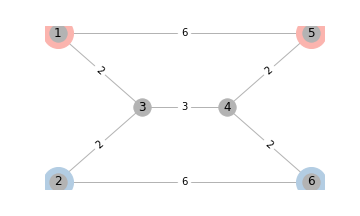
\includegraphics[width=6cm]{../resources/example_1_base.png}
    \caption{Representacón de la red utilizada para el ejemplo 1. Los dos pares origen destino se detallan con un color diferente cada uno. Cada arco tiene una etiqueta con el costo de usuario sobre la infrastructura base, es decir, la red de calles.}
    \label{fig:example1base}
  \end{figure}

  Podemos deducir rápidamente en la figura de la red (\ref{fig:example1base}) que el camino más corto para ambos pares origen destino sobre la red de calles de 1 arco y de costo 6. El objetivo entonces es decidir dónde construir infrastructuras 1 tal que el costo de los caminos más cortos de uno o ambos pares origen-destino sea menor a 4 (dado por la función de transferencia de demanda) de manera que una cantidad $D$ o $2D$ de demanda sea transferida a la bicicleta. Si decidimos utilizar infrastructura 1 en alguno de los arcos (1, 5) o (2, 6), digamos el primero, entonces nos aseguramos que la demanda del par origen-destino (1, 5) sera transferida a la bicicleta ya que su nuevo costo del camino más corto pasa a ser $3$. Con el presupuesto remanente de $5$, solo podremos construir infrastructura 1 en a lo sumo dos de los arcos (2, 3), (3, 4) y (4, 5). No es dificil ver que a lo sumo podremos mejorar el costo del camino más corto a $4.5$ para el par origen destino (2, 6). La demanda transferida total en este caso es entonces de $D$.

  La solución óptima viene de construir infrastructura 1 en todos los arcos del grafo menos los (1, 5) y (2, 6). Esto permite que ambos pares origen destino tengan un nuevo recorrido como camino más corto, de costo $3.5$, lo que permite, según la función de transferencia de demanda, transferir $2D$ unidades de demanda. Esta solución se puede observar gráficamente en la figura (\ref{fig:example1solution}).

  \begin{figure}[h!]
    \centering
    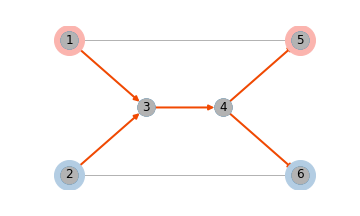
\includegraphics[width=6cm]{../resources/example_1_infras.png}
    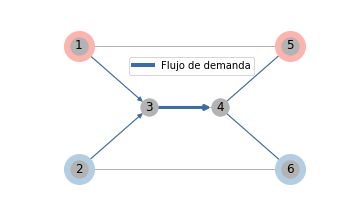
\includegraphics[width=6cm]{../resources/example_1_flows.png}
    \caption{Representacón de la solución óptima en el grafo. A la izquierda se muestra en naranja en cuáles arcos se construye la infrastructura 1. A la derecha, los flujos sobre los caminos más cortos para ambos pares origen-destino, en azul, nótese que el ancho del arco en este caso da una noción de la cantidad flujo.}
    \label{fig:example1solution}
  \end{figure}

  Para mostrar que la solución es óptima para la formulación binivel, podemos decir que no hay asignación de infrastructuras a arcos que induzcan una demanda transferida mayor dado los caminos más cortos encontrados para cada par origen-destino, para cada otra asignación posible analizada.
  Este ejemplo trivial nos da una idea de la complejidad combinatoria que tiene este problema. Supongamos que a la red existente se le agregan aleatoriamente 100 nodos y arcos de alto costo de usuario suficientes para lograr que sea 4-conexo, por decir algo, entonces tendríamos que la solcuión óptima es la misma, pero esta vez deberiamos analizar mucho mas posibilidades, dada la naturaleza compartida de las infrastructuras de ciclovía.

  Finalmente, una dificultad intrínseca de las formulaciones binivel es que no existen maneras de resolverlos directamente con un solver por lo que luego analizaremos maneras de reformular el planteo y analizar formulaciones alternativas.

  \subsection*{Algunas hipótesis}

  En este trabajo asumimos las siguientes hipótesis que entedemos tienen sentido en este contexto:

  \begin{itemize}
    \item{El tiempo de viaje en todo arco de la red es independiente del flujo sobre el mismo.}
    \item{Existen diferentes pares origen-destino en la red, cada uno con un valor de demanda, y para cada origen y destino existen potencialmente diferentes caminos que unen el origen y el destino.}
    \item{Los usuarios siempre buscan minimizar el costo de su viaje (todos son
    perfectos optimizadores y se comportan igual)}
  \end{itemize}

  Sobre la red, consideramos que los grafos son dirigidos y cuando se decide construir una infraestructura sobre un arco solo se hace en la dirección del arco. Esto simplifica el modelado pero puede no ser tan realista considerando que el costo marginal de construir una infraestructura dado que existe la misma infraestructura en el otro sentido es menor al costo de construir la primera. Tambien puede resultar en que dado dos nodos adyacentes mutuamente, se decida construir diferentes infraestructuras en cada sentido. Sin embargo, dado que en general las redes que modelan las ciudades sobre las que se quieren resolver estos problemas son una simplificación de la red de calles, las consideraciones irreales mencionadas no tienen consecuencia práctica.

  La formulación que planteamos considera aspectos de modelos descriptivos en donde el objetivo es simular el comportamiento de los usuarios, y modelos normativos (o de optimización) en donde el objetivo es mejorar las decisiones que afectan un proceso. TODO: Referencias y mencion sobre complejidad de mezclar ambos.

  \subsection*{Características de una solución}

  Como marco para para evaluar la validez del modelo definimos algunas características deseables que, entendemos, deben cumplir una solución del problema, cuya formulación puede ser desconocida a estos efectos.

  Consideramos que una solución cumple los siguientes puntos:

  \begin{enumerate}
      \item{El costo de los caminos más cortos entre pares origen-destino sobre la red resultante, es decir adicionando infrastructuras, es menor o igual al costo sobre la red sin infraestructuras.}
    \item{\label{budgetexcess} El presupuesto excedente no es suficiente para agregar una infraestructura que mejore el costo de alguno de los caminos más cortos.}
    \item{El camino más corto sobre la red resultante para un par origen-destino no puede inducir un valor de demanda transferida distinto al de la solución.}
  \end{enumerate}

  \subsection*{Formulación matemática}

  Finalmente presentamos la formulación matemática formal. Sean:

  \begin{description}
    \item[$OD$]: Conjunto de pares origen destino con elemento genérico $k$.
    \item[$G=(N,A)$]: Grafo dirigido que modela la red, con su conjunto de nodos $N$ y de arcos $A$. $A_n^+$ y $A_n^-$ son los conjuntos de arcos que salen y entran respectivamente desde el nodo $n$.
    \item[$I$]: Conjunto de infraestructuras de ciclovías.
    \item[$C_{ai}$]: Costo de usuario de atravesar el arco $a \in A$ utilizando la infraestructura $i \in I$. $C_{ai} > 0$.
    \item[$H_{ai}$]: Costo de construcción de la infraestructura $i \in I$ en el arco $a \in A$. $H_{ai} \geq 0$ .
    \item[$B$]: Presupuesto para la construcción de infraestructuras.
    \item[$\theta_{nk}$]: Parámetro que vale 1 si n es el origen del par origen-destino $k \in OD$, -1 si es el destino y 0 en otro caso.
    \item[$w_k$]: Variable de primer nivel que contiene el valor del camino más corto para el par origen destino $k \in OD$.
    \item[$y_{ai}$]: Variable binaria de primer nivel que determina si la infraestructura $i \in I$ está activa en el arco $a \in A$.
    \item[$x_{ak}$]: Variable de segundo nivel que determina si el arco $a \in A$ es parte del camino más corto para el par origen-destino $k \in OD$.
    \item[$f_k$]: Función que determina la demanda que utiliza la bicicleta como modo de transporte en función del costo del camino mas corto.
  \end{description}

  Definimos la siguiente formulación de programación matemática:

  \begin{align}
    \text{max}    & \sum_{k \in OD} f_k(w_k)                                                         & \label{eq:objective1lvl} \\
    \text{s.t.}\; & w_k = \sum_{a \in A} \sum_{k \in OD} \sum_{i \in I} C_{ai}y_{ai}x_{ak}           & \forall k \in OD \label{eq:shortestpath} \\
                  & B \geq \sum_{a \in A} \sum_{i \in I} H_{ai}y_{ai}                                & \label{eq:respectbudget} \\
                  & 1 = \sum_{i \in I} y_{ai}                                                        & \forall a \in A \label{eq:alwaysoney} \\
                  & w_k \geq 0, y_{ai} \in \{0,1\}                                                   & \nonumber \\
                  & \text{min} \sum_{a \in A} \sum_{k \in OD} \sum_{i \in I} C_{ai}y_{ai}x_{ak}      & \label{eq:subproblem} \\
                  & \text{s.t.} \sum_{a \in A_n^+} x_{ak} - \sum_{a \in A_n^-} x_{ak} = \theta_{nk}  & \forall n \in N, k \in OD \label {eq:flowbalance} \\
                  & \modelspace x_{ak} \geq 0                                                        & \nonumber
  \end{align}

  Donde:

  \begin{description}
    \item[\ref{eq:objective1lvl}]: La función objetivo es la suma de los valores de demandas que cambiaron de modo de transporte.
    \item[\ref{eq:shortestpath}]: Restricción que determina el costo del camino más corto dado en el primer nivel.
    \item[\ref{eq:respectbudget}]: Restricción de presupuesto sobre lo que se puede construir.
    \item[\ref{eq:alwaysoney}]: Restricción que requiere que una infraestructura estar activa en cada arco. Se discutirá más sobre esto en la siguiente sección.
    \item[\ref{eq:subproblem}]: Función objetivo del segundo nivel.
    \item[\ref{eq:flowbalance}]: Restricción de balance de flujo.
  \end{description}

  \subsubsection*{Observaciones}

  La linealidad de la formulación propuesta es determinada por las funciónes $f_k$. En las ecuaciones (\ref{eq:shortestpath}) y (\ref{eq:subproblem}) las variables de primer y segundo nivel se multiplican pero dado que las variables de un nivel son parámetro en el otro nivel no se pierde la linealidad de dichas ecuaciónes.

  En la formulación del problema de primer nivel, la restricción (\ref{eq:alwaysoney}) pudo haber sido escrita de manera que a lo sumo una infraestructura esté activa, es decir dejar la posibilidad de que no haya infrastructuras activas en un arco. Esto se puede ver de diferentes maneras, pensando en la realidad modelada, un ciclista podría pasar prácticamente por cualquier calle sin problemas, entonces para que las instancias del modelo sean semánticamente correctas debería existir una infraestructura $i_0 \in I$ cuyo costo de construcción $H_{ai_0}$ sea 0 en todos de los arcos $a \in A$, mas allá de que el costo de usuario pueda ser altísimo. Desde un punto de vista formal, como se verá mas adelante, si no se requiere que en cada arco haya una infraestructura activa, entonces se debe agregar al problema de segundo nivel una restricción que evite que se activen flujos en arcos donde no hay infraestructura activa, es decir: $x_{ak} \leq \sum_{i \in I} y_{ai}, \forall a \in A, k \in OD$. Con esta restricción, el problema de segundo nivel puede no tener solución factible cuando las infraestructuras seleccionadas por el primer nivel no inducen un subgrafo que conectan todos los pares origen-destino.

  Asumiremos de aquí en adelante que las instancias del problema están bien definidas, esto significa que:

  \begin{enumerate}
    \item {$G$ es conexo}
    \item {$\forall k \in OD$ existe un camino $S_k \in G$ con costo de construcción cero, es decir $\sum_{a \in S_k} H_{ai_0} = 0$}
  \end{enumerate}

  \section*{Consideraciones semánticamas}

  Es de nuestro particular interés para la formulación los parámetros que representan la demanda y funciones de transferencia de demanda entre modos. Se incurre en una simplificación que reduce varios modos de transporte, por ejemplo transporte público, taxi o privado; a uno y consideramos la transferencia desde este modo agregado a la bicicleta. Por otro lado, las funciones de transferencia de demanda son funciones de $R^+$ en $R^+$, cuyo dominio está en unidad del costo de usuario y su codominio en unidad de demanda.

  \subsection*{Transferencia de demanda}

  El modelo busca determinar la mayor transferencia de demanda entre dos modos de transporte. Para esto, consideramos que, sobre la infrastructura base, la demanda transferida es cero, es decir, que el costo del camino más corto utilizando la bicicleta sobre únicamente la infrastructura base no induce transferencia de demanda a la bicicleta. Suponemos que partimos de un conjunto de demanda insatisfecha por la infrastructura ciclovias base, pero potencial, si las condiciones mejoran.

  En la práctica, la decisión de utilizar la bicicleta es multifactorial y dependen altamente en tres tipos de factores:

  \begin{enumerate}
    \item{
        Características del viajante
          \begin{itemize}
            \item{Edad}
            \item{Nivel socioeconómico}
            \item{Otros factores como utilización de auto para el trabajo, llevar niños a escuela, etc.}
          \end{itemize}
    }
    \item{
        Características del viaje
          \begin{itemize}
            \item{Propósito}
            \item{Momento del día}
          \end{itemize}
    }
    \item{
        Características quantitativas y cualitativas de las facilidades de transporte
        \begin{itemize}
            \item{Disponibilida de transporte público}
            \item{Infrastructuras de ciclovías}
            \item{Costo de boleto y combustibles}
            \item{Comodidad y conveniencia}
            \item{Seguridad y proyección}
        \end{itemize}
    }
  \end{enumerate}

  En este trabajo nos concentramos en el último punto exclusivamente. Mediante la construcción de ciclovías, se podrán obtener mejoras en varios de estos puntos, que modelamos como un único valor. Sobre los otros factores, asumimos que solo consideramos el universo de demanda que es trasnferible a la bicicleta, esto nos ahorra considerar aspectos como: si el viaje se hace de noche o si mi trabajo requiere un vehículo automotor.

  \subsection*{Validación de la formulación}

  Para discutir la validez matemática del modelado partimos de una formulación estándar de problema binivel o BLPP (Bi Level Programming Problem), como se puede encontrara en Bard (\ref{bardbook}).

  Sea la siguiente formulación simplificada del problema:

  \begin{align}
    \text{max}_{y \in Y}    & \; F(x, y) \label{bilevelgeneric1} \\
    \text{s.t.} \modelspace & A_1 x + B_1 y \leq b_1 \\
                            & y \geq 0 \\
                            & \text{min}_{x \in X} f(x, y) \\
                            & \modelspace A_2 x + B_2 y \leq b_2 \label{bilevelgeneric5} \\
                            & \modelspace x \geq 0 \label{bilevelgeneric6}
  \end{align}

  Y las siguientes definiciones:

  \begin{definition}
    Conjunto factible
    \begin{align}
      S = \{(x, y) \setminus x \in X, y \in Y, A_1 x + B_1 y \leq b_1, A_2 x + B_2 y \leq b_2 \}
    \end{align}
  \end{definition}

  \begin{definition}
    Conjunto de reacción del segundo nivel:
    \begin{align}
      P(y) = \{ x \in \text{argmin}_{\hat{x} \in X} f(\hat{x}, y) : A_2 \hat{x} + B_2 y \leq b_2 \}
    \end{align}
  \end{definition}

  Diremos que el problema está bien formulado si el conjunto $S$ es no vacío, es decir, si existen soluciones factibles y si para toda $y$ el conjunto $P(y)$ es no vacío, es decir, si para todo movimiento del problema de primer nivel, hay margen de decisión en el segundo nivel.

  \begin{lemma}$S$ es no vacío
  \end{lemma}

  \begin{proof}
    $S \neq \emptyset$ ya que $\exists (x_0, y_0) \in X \times Y$ donde $y_0$ es el vector $y_{ai_0} = 1 \forall a \in A$, $i_0$ es la infraestructura cuyo costo $H_{ai_0} = 0$, lo que deja al resto de las entradas del vector $y_0$ en $0$. Por lo tanto se cumple las restricción (\ref{eq:alwaysoney}) dado que todos los arcos tienen una infraestructura activa, y la restricción (\ref{eq:respectbudget}) dado que el costo total de construcción de $y_0$ es $0$.

    Luego, dado que las infraestructuras activas logran la conectividad de los pares origen-destino y el hecho de que el el costo de los arcos $C_ai$ sea no negativo permite asegurar que el problema de segundo nivel tiene al menos una solución factible $x_0$.
  \end{proof}

  \begin{lemma}$\forall y \in Y,\; P(y) \neq \emptyset$
  \end{lemma}

  \begin{proof}
    Para cualquier asignación $y = \hat{y} \in Y$, se cumple que $P(\hat{y})$ es no vacío ya que todos los arcos tienen una infraestructura activa, por lo tanto el grafo donde los flujos del problema de segundo nivel pueden pasar es conexo y llega necesariamente a todos los nodos, incluyendo los pares origen-destino. Por lo tanto el espacio de soluciones factibles del subproblema es no vacío. 
  \end{proof}

  Aún cuando estas dos definiciones se cumplen, puede haber dificultades al encontrar la solución óptima cuando $P(y)$ contiene más de un elemento, caso en el cual el modelo puede no llegar a la solución óptima, dependiendo del valor $x \in P(y)$ que seleccione el problema de segundo nivel. En este caso de estudio esto es muy probable que suceda, puesto que pueden haber varios caminos más cortos entre dos puntos.

  \section*{Resolución del problema}

  Si bien la formulación binivel expresa de buena manera lo que queremos resolver, en la práctica los BLPP son en general de dificil resolución, ya se ha demostrado en Bard (\ref{bardbook}) que el BLPP lineal en su formulación general es es NP-Hard. Además los métodos existentes para su transformación a formulaciones de un nivel no son directos. En esta sección mencionamos la metodología más común, que consiste en sustituir el problema del segundo nivel por las condiciones de optimalidad de KKT. Luego analizaremos una formulación alternativa cuya equivalencia con el problema binivel está condicionada a este problema en particular. Previo a estos dos análisis debemos reacomodar la formulación binivel de manera que las variables de diferente nivel no se encuentren en un producto ya que esto deviene en restricciónes no lineales luego de las transformaciones.

  \subsection*{Transformación de binivel a un nivel}

  Este problema se puede transformar a un problema de un nivel sustituyendo el problema de segundo nivel por sus restricciónes de optimalidad de KKT en el primer nivel. De obtenerse una representación lineal se podría buscar alguna metodología exacta para resolverlo. La formulación binivel estudiada presenta el problema, a los efectos de la transformación, de contener ecuaciones con variables de diferentes niveles multiplicándose, dichas ecuaciones deben ser reformuladas para que no devengan en restricciones no lineales.

  \subsection*{Quitando producto de variables $x_{ak}$ e $y_{ai}$}

  Se propone la siguiente formulación del problema de segundo nivel:

  \begin{align}
    \text{min}  & \sum_{k \in K} \sum_{a \in A} \sum_{i \in I} C_{ai} h_{aki}         & \label{eq:subproblemrefeq1} \\
    \text{s.t.} & \sum_{a \in A_n^+} x_{ak} - \sum_{a \in A_n^-} x_{ak} = \theta_{nk} & \forall n \in N, k \in OD \\
                & 0 \leq h_{aki} \leq y_{ai}                                          & \forall a \in A, k \in K, i \in I \\
                & x_{ak} = \sum_{i \in I} h_{aki}                                     & \forall a \in A, k \in K
  \end{align}

  Si utilizamos la ecuación (\ref{eq:subproblemrefeq1}) en la restricción de igualdad de $w_k$ (ecuación \ref{eq:shortestpath}) el problema es equivalente con la ventaja que no existen variables de diferentes niveles multiplicándose. La equivalencia se da porque esta formulación desagrega los flujos para cada infraestructura ademas de par origen-destino y arco en la variable $h_{aki}$, que es lo que se modela con el producto $y_{ai} x_{ak}$.

  \subsection*{Transformación por condiciones de KKT}

  Sea la formulación generica binivel (\ref{bilevelgeneric1})-(\ref{bilevelgeneric6}), y sea $f(x, y) = cx + dy$, entonces podemos sustituir el problema de segundo nivel por sus condiciones de optimalidad de KKT agregando las variables $v$ y $u$ de la siguiente manera:

  \begin{align}
    \text{max}              & \; F(x, y) \label{kktgeneric1} \\
    \text{s.t.}             & A_1 x + B_1 y \leq b_1 \\
                            & uB_2 - v = -c \\
                            & u(b_2 - A_2x - B_2y) + vx = 0 \label{kktgeneric_complslack} \\
                            & A_2 x + B_2 y \leq b_2 \label{kktgeneric5} \\
                            & x, y, v, u \geq 0 \label{kktgeneric6} \\
  \end{align}

  La restricción (\ref{kktgeneric_complslack}) es problemática dado que el objetivo es resolver el problema con un solver lineal. Aplicando el teorema de holgura complementaria sabemos que ambos sumandos son 0. Luego, podemos reemplazar la restricción $u(b_2 - A_2x - B_2y) = 0$ por dos conjuntos de restricciones equivalentes, agregando variables binarias $z$ y una constante $M$ suficientemente grande, de manera que quede: $u \leq Mz$ y $b_2 - A_2x - B_2y \leq M(1-z)$.

  Si aplicamos esta transformación a nuestro problema binivel, tendriamos que agregar $|N| |OD|$ variables binarias, que, considerando las ya existentes variables $y_{ai}$ y las que agregaremos por temas intrínsecos del problema entendemos que supone una complejidad inncecesaria, dada la formulación alternativa que analizaremos a continuación.

  \subsection*{Formulación alternativa de un nivel}
  \label{altOneLevelFormulation}

  A diferencia de la transformación a un nivel que podemos decir que resulta en una formulación equivalente a la binivel, en esta sección proponemos una formulación alternativa que entendemos equivalente en el sentido de lo que queremos resolver y obtener de la resolución, es decir, un valor de demanda transferida y un conjunto de decisiones de cuales infrastructuras construir y dónde.

  Esta formulación nace de la formulación binivel quitando el subproblema y agregando sus restricciones al problema de primer nivel bajo el argumento de que las funciones $f_k$ deben ser decrecientes para que el problema tenga sentido semánticamente. Dado lo anterior, para maximizar $\sum_{j \in OD}f_k(w_k)$ lo mejor es los $w_k$ sean lo más chico posible.

  La formulación resultante es la siguiente:

  \begin{align}
    \text{max}    & \sum_{k \in OD} f_k(w_k)                                                         & \label{eq:objectivealt} \\
    \text{s.t.}\; & w_k = \sum_{a \in A} \sum_{k \in OD} \sum_{i \in I} C_{ai}y_{ai}x_{ak}           & \forall k \in OD \label{eq:shortestpathalt} \\
                  & B \geq \sum_{a \in A} \sum_{i \in I} H_{ai}y_{ai}                                & \label{eq:respectbudgetalt} \\
                  & 1 = \sum_{i \in I} y_{ai}                                                        & \forall a \in A \label{eq:alwaysoneyalt} \\
                  & \sum_{a \in A_n^+} x_{ak} - \sum_{a \in A_n^-} x_{ak} = \theta_{nk}              & \forall n \in N, k \in OD \label{eq:flowbalancealt} \\
                  & w_k \geq 0, x_{ak} \geq 0, y_{ai} \in \{0,1\}                                    & \nonumber
  \end{align}

  \subsubsection*{Observaciones}

  La formulación en realidad asume que las funciones $f_k$ son estrictamente decrecientes. Notaremos que si las funciones son solo decrecientes, entonces puede haber valores de costos de caminos más cortos que no tienen insentivo a decrecer. No vamos a imponer esta restricción sobre las funciones de transferencia de demanda, sino que analizaremos variantes de esta formulación como multiobjetivo lexicográfico.

  \subsection*{Definición de las $f_k$s}

  TODO: POR ACA VOY EN EL REPASO

  Estas funciones fueron dejadas de lado en la formulación inicial con el objetivo de analizar las restricciones principales primero. Se analizan en esta sección diferentes alternativas de cómo implementarlas como un conjunto de ecuaciones lineales que se acoplaran a las formulación antedicha.

  Podemos encontrar en la literatura soluciones a problemas similares. En Laporte 2007 (\ref{laporte2007}) y Lim 2021 (\ref{lim2021}), donde se considera un parámetro $c^{PRIV}_k$ que modela el costo del transporte privado para un par origen-destino $k$, si la red de transporte público logra un costo menor entonces se considera que toda la demanda del par origen-destino $k$ se transfiere a dicho modo.

  \subsubsection*{Definición propuesta}

  Se considera que una función $f_k$ arbitraria debe poder modelar una transición paulatina de la demanda entre modos de transporte. Paulatina de manera de expresar una transición que pueda parecerse a algo lineal, exponencial o lo que fuere. Asumiendo que las $f_k$ son decrecientes, la mejor forma que ocurriese es representarla como una sucesión decreciente de puntos de quiebre, tal que para cada uno se exista un valor asociado de cantidad de demanda transferida. Los puntos de quiebre son comparados contra el valor del camino más corto $w_k$. Entonces sea $w_k$ fijo, la demanda transferida es:

  \begin{equation}
    \label{eq:deffks}
    f_k(w_k) = P_{j^*},\; j^* = argmin_{j \in J} \{Q_j \geq w_k\}
  \end{equation}
  
  Donde $Q_j$ son los puntos de quiebre en la unidad del costo del camino más corto, $J$ es un conjunto índice y $P_{j^*}$ es la cantidad de demanda que se transfiere. Una ventaja de esta formulación es que puede ser integrada a la función objetivo de la formulación inicial de manera que la minimización queda en manos del objetivo del mismo problema.

  Como alternativa, se puede podría pensar una definición de $f_k$ como función no lineal, esto puede llevar a soluciones soluciones analíticamente más precisas pero es sabido que aumenta considerablemente la dificultad de resolución práctica.

  Para modelar la función $argmin$ en una formulación como la que se viene trabajando es necesario utilizar variables de activación que solo permita que una entrada del índice esté activo. Por ejemplo si se usa $z_j,\; j \in J$, lo antedicho equivale a decir que $z_j \in \{0,1\}$ y $\sum_{j \in J} z_j = 1$. Como estas restricciones se encuentran dentro de una maximización y suponiendo que el conjunto ordenado $Q$ es estrictamente decrecientes, podemos relajar la restricción de integralidad y sustituirla por $0 \leq z_j \leq 1$. Es esperable pensar que no pueden existir varios $z_j$ activos para la definición (\ref{eq:deffks}), porque si los hubiesen, al ser $Q$ y $P$ conjuntos ordenados estrictamente decreciente entonces no se llegaría al máximo.

  Nótese que esta definición es una extensión de la propuesta por Laporte 2007 (\ref{laporte2007}) y Lim 2021 (\ref{lim2021}). Para modelarla basta considerar $J = \{0, 1\}$, $P_0 = 0, P_1 = D_k$ y $Q_0 = M, Q_1 = c^{PRIV}_k$, donde $M$ es un numero arbitrario mayor a $c^{PRIV}_k$ y $D_k$ es la demanda para el par origen-destino $k$.

  \subsubsection*{Formulación de $f_k$ como LP}

  En esta sección se discuten diferentes formulaciones de $f_k$ como LP con el objetivo de analizar cómo se integrará a la formulación del problema que se quiere resolver. La forma más simple de modelar $f_k$ (ó simplemente $f$) es la (\ref{eq:fkv1eq1})-(\ref{eq:fkv1eq4}).

  \begin{align}
    f(W) =\; & max \sum_{j \in J} P_j y_j    & \label{eq:fkv1eq1}\\
             & s.t. \sum_{j \in J} y_j = 1   & \label{eq:fkv1eq2} \\
             & \;\;\; Q_j \geq W y_j         & \label{eq:fkv1eq3} \forall j \in J \\
             & \;\;\; y_j \in \{0,1\}        & \label{eq:fkv1eq4}
  \end{align}

  Si se intenta integrar esta formulación a (\ref{eq:objective1lvlfinal})-(\ref{eq:respectinfra}) el resultado seria un problema quadrático ya que $W$ sería sustituido por $w_k$. Por este motivo se estudiaron dos formulaciones alternativas que logran solucionar esta situación. La idea en ambas es desagregar $W$ como la suma de nuevas variables y utilizar estas en la restricción (\ref{eq:fkv1eq3}) en lugar de $W y_j$.

  \paragraph*{$f_k$ como LP version 1}

  \begin{align}
    f(W) =\; & max \sum_{j \in J} P_j y_j             & \label{eq:fkv3eq1}\\
             & s.t. \sum_{j \in J} y_j = 1            & \label{eq:fkv3eq2}\\
             & \;\;\; Q_j \geq w^{aux}_j              & \forall j \in J \label{eq:fkv3eq3} \\
             & \;\;\; w^{aux}_j \leq M y_j            & \forall j \in J \label{eq:fkv3eq4} \\
             & \;\;\; w^{sink}_j \leq M (1 - y_j)     & \forall j \in J \label{eq:fkv3eq5} \\
             & \;\;\; w^{sink}_j + w^{aux}_j = W      & \label{eq:fkv3eq6} \\
             & \;\;\; y_j \in \{0,1\}                 & \label{eq:fkv3domainy} \\
             & \;\;\; w^{aux}_j, w^{sink}_j \geq 0    & \label{eq:fkv3eq7}
  \end{align}

  Se desagrega $W$, para cada $j$ en $w^{sink}_j + w^{aux}_j$ de manera que uno de los dos tenga el valor de $W$, esto se logra con las restricciones (\ref{eq:fkv3eq4}) y (\ref{eq:fkv3eq5}). Entonces se cumple que solo el $w^{aux}_j$ cuyo $y_j$ esté activo tendrá el valor de $W$. Las mencionadas restricciones sirven para activar $y_i$ utilizado un parámetro $M \geq W$ arbitrario. Finalmente las restricciónes (\ref{eq:fkv3eq2}) y (\ref{eq:fkv3eq6}) logran que solo una de las variables $w^{aux}_j$ o $w^{sink}_j$ tome el valor de $W$, para cada $j$.

  \paragraph*{$f_k$ como LP version 2}

  \begin{align}
    f(W) =\; & max \sum_{j \in J} P_j y_j             & \label{eq:fkv2eq1}\\
             & s.t. \sum_{j \in J} y_j = 1            & \label{eq:fkv2eq2}\\
             & \;\;\; Q_j \geq w^{aux}_j              & \forall j \in J \label{eq:implfkoriginalineq} \\
             & \;\;\; w^{aux}_j \leq M y_j            & \forall j \in J \label{eq:yactivation1} \\
             & \;\;\; \sum_{j \in J} w^{aux}_j = W    & \label{eq:activatewaux} \\
             & \;\;\; y_j \in \{0,1\}                 & \label{eq:fkv2domainy} \\
             & \;\;\; w^{aux}_j \geq 0                & \label{eq:fkv2eq6}
  \end{align}

  En este caso se desagrega $W$ como suma de $|J|$ variables $w^{aux}_j$ de manera que solo una de ellas esté activa y tenga el valor de $W$. Para activar $y_i$ se agrega la restricción (\ref{eq:yactivation1}) utilizado, igual que en la formulación anterior, un parámetro $M \geq W$ y finalmente las restricciónes (\ref{eq:activatewaux}) y (\ref{eq:fkv2eq2}) logran que solo uno de los $w^{aux}_j$ tome el valor de $W$ y el resto sean 0.

  \subsubsection*{Validación de la formulación}

  Según definimos $f_k(W)$ en (\ref{eq:deffks}), sea de $p = f_k(W)$, entonces se cumple que:

  \begin{enumerate}
    \item {\label{deffpt1} $p$ es exactamente uno de los valores del conjunto de valores $P_j$, es decir: $p \in \{P_j\}_{j \in J}$}
    \item {\label{deffpt2} Sea $\hat{j} = j \;|\; p = P_j$. El valor del punto de quiebre $Q$ asociado a $\hat{j}$ no es menor que el costo del camino más corto $W$, es decir: $Q_{\hat{j}} \geq W$.}
    \item {\label{deffpt3} Dado el $\hat{j}$ anterior, entonces no existe un punto de quiebre $Q_j \forall j \in J$ que sea no mayor al punto de quiebre $Q_{\hat{j}}$ y mayor o igual al costo del camino más corto, es decir: $\not{\exists}\; Q_j\; \forall j \in J \;|\; Q_j \in  [W, Q_{\hat{j}}]$}.
  \end{enumerate}

  Es de interés analizar la correctitud de las formulaciones respecto a los puntos mencionados. En particular, la versión 2 (\ref{eq:fkv2eq1}) - (\ref{eq:fkv2eq6}) que es la que se utilizará finalmente. Se tiene que el punto \ref{deffpt1} se cumple, en la formulación, en la función objetivo (\ref{eq:fkv2eq1}) donde el valor objetivo es la suma de un subconjunto de $\{P_j\}_{j \in J}$, la restricción (\ref{eq:fkv2eq2}) que dice que solo uno de esos valores puede estar activo en la suma del objetivo y la restricción (\ref{eq:fkv2domainy}) que determina el carácter de la variable de decisión. El punto \ref{deffpt2} se cumple en la restricción (\ref{eq:implfkoriginalineq}), dado que $w^{aux}_j$ es igual a $W$ o cero, como se detalla en las restricciones (\ref{eq:yactivation1}), (\ref{eq:activatewaux}) y el carácter binario de $y_j$. Si $w^{aux}_j = W$, entonces el $j$ activo es el valor funcional de $f(W)$ y se cumple la definición del punto \ref{deffpt2}. Por otro lado, si es cero entonces el $j$ activo no es $\hat{j}$ y por lo tanto también se cumple el punto en cuestión. Finalmente, el punto \ref{deffpt3} se cumple por el hecho de que la función objetivo es una maximización y que $f(W)$ es una función estrictamente decreciente, entonces si existiera un $Q_a \in \{Q_j\}_{j \in J} \;|\; Q_a < Q_{\hat{j}}, a \in J$ entonces por se $f$ decreciente existe un valor $P_a > P_{\hat{j}}$ lo que contradice el hecho mismo de que el objetivo sea una maximización.

  \subsubsection*{Valores posibles de $P_j$ y $Q_j$}

  Para un $k \in OD$, sea $\overline{W}$ el costo del camino más corto sobre el grafo base (sin infraestructuras) y $\underline{W}$ el mejor costo del camino más corto suponiendo que las mejores infraestructuras se pueden construir, entonces $Q_j \in [\underline{W}, \overline{W}],\; \forall j \in J$\footnote{En realidad, $\overline{W}$ es el mínimo valor para el que $f_k$ es mínimo, podría ser cualquier numero arbitrariamente grande.}. Los valores de $Pj$ son la cantidad de demanda que se transfiere para cada $Q_j$ y dependen del par origen-destino $k$.

  Una forma posible de establecer los valores de $J$, $P_j$ y $Q_J$ es, dada una aproximación continua de $f_k$, tomando $N$ valores equidistantes entre $[\underline{W}, \overline{W}]$ obtendremos $Q_j$, y tomando el valor funcional de esos puntos obtendremos $P_j$, luego $J=\{1,..,N\}$. Es deseable también que el mínimo de $f_k$ sea 0, es decir, que si ninguna mejora es impuesta al camino más corto no haya transferencia de demanda.

  TODO: mencionar que en la mayor parte de los estudios se enfoca en sistemas de bicicletas compartidos y que el modelado de transferencia de demanda no es gradual como en este trabajo. Con referencias obvio.

  \section*{Poniendo todo junto}

  Se escribe aquí las formulaciónes completas del problema en su forma binivel y su alternativa de un nivel, agregando las definiciones de $f_k$ y quitando la multiplicación de variables. TODO: redondear esta parte que es importante para la seccion de perturbacion de parametros.

  \subsection*{Formulación binivel}

  Además de las definiciones en la formulación inicial (\ref{eq:objective1lvl})-(\ref{eq:flowbalance}):

  \begin{description}
    \item[$J$]: Es un conjunto índice utilizado en los conjuntos $P$ y $Q$.
    \item[$P_{kj}$]: Parámetro que determina la cantidad de demanda transferida para el par origen-destino $k \in OD$ y el índice $j \in J$.
    \item[$Q_{kj}$]: Parámetro que contiene el punto de quiebre para determinar la demanda transferida para el par origen-destino $k \in OD$ e índice $j \in J$.
    \item[$M$]: Número positivo muy grande. 
    \item[$z_{kj}$]: Variable binaria que determina si demanda transferida para el par origen-destino $k \in OD$ es la de índice $j \in J$.
    \item[$h_{aki}$]: Variable no negativa que determina el flujo que pasa por el arco $a \in A$, para el par origen-destino $k \in OD$ utilizando la infraestructura $i \in I$.
    \item[$w^{aux}_{kj}$]: Variable no negativa que contiene el valor de $w_{k}$ si $z_{kj}$ esta activa y cero sino. 
  \end{description}

  \begin{align}
    \text{max}    & \sum_{k \in OD} \sum_{j \in J} P_{kj} z_{kj}                                     & \label{eq:objective1lvlfinal} \\
    \text{s.t.}\; & w_k = \sum_{a \in A} \sum_{i \in I} C_{ai}h_{aki}                                & \forall k \in OD \label{eq:shortestpathfinal} \\
                  & Q_{kj} \geq w^{aux}_{kj}                                                         & \forall j \in J, k \in OD \label{eq:breakpoints} \\
                  & w^{aux}_{kj} \leq M z_{kj}                                                       & \forall j \in J, k \in OD \\
                  & \sum_{j \in J} w^{aux}_{kj} = w_k                                                & \forall k \in OD \\
                  & \sum_{j \in J} z_{kj} = 1                                                        & \forall k \in OD \label{eq:singularbreakpoint} \\
                  & B \geq \sum_{a \in A} \sum_{i \in I} H_{ai}y_{ai}                                & \label{eq:respectbudgetfinal} \\
                  & 1 = \sum_{i \in I} y_{ai}                                                        & \forall a \in A \label{eq:alwaysoneyfinal} \\
                  & w_k \geq 0, y_{ai} \in \{0,1\}, z_{kj} \in \{0,1\}                               & \nonumber \\
                  & \text{min} \sum_{k \in K} \sum_{a \in A} \sum_{i \in I} C_{ai} h_{aki}           & \label{eq:subproblemfinal} \\
                  & \text{s.t.} \sum_{a \in A_n^+} x_{ak} - \sum_{a \in A_n^-} x_{ak} = \theta_{nk}  & \forall n \in N, k \in OD \label{eq:flowbalancefinal} \\
                  & \modelspace x_{ak} = \sum_{i \in I} h_{aki}                                      & \forall a \in A, k \in K \label{eq:flowactivation} \\
                  & \modelspace 0 \leq h_{aki} \leq y_{ai}                                           & \forall a \in A, k \in K, i \in I \label{eq:respectinfra} \\
                  & \modelspace x_{ak} \geq 0, h_{aki} \geq 0                                        & \forall a \in A, k \in K \nonumber
  \end{align}

  Donde las nuevas ecuaciones son:

  \begin{description}
    \item[\ref{eq:objective1lvlfinal}]: Función que suma los valores de demanda transferida $P_{kj}$ activos.
    \item[\ref{eq:breakpoints}]: Restricción que determina que los puntos de quiebre activos son aquellos cuyo costo es menor o igual al del camino más corto.
    \item[\ref{eq:singularbreakpoint}]: Restricción que permite solo un punto de quiebre activo para cada par origen-destino $k \in OD$.
    \item[\ref{eq:flowactivation}]: El flujo total para el arco $a \in A$ y el par origen-destino $k \in OD$ es la suma de los flujos de todos las infraestructuras.
    \item[\ref{eq:respectinfra}]: El flujo por el arco $a \in A$, para el par origen-destino $k \in OD$ y la infraestructura $i \in I$ puede estar activo si la infraestructura $i$ esta activa.  
  \end{description}

  \subsection*{Formulación de un nivel}

  \begin{align}
    \text{max}    & \sum_{k \in OD} \sum_{j \in J} P_{kj} z_{kj}                          & \label{eq:objectivealtfinal} \\
    \text{s.t.}\; & w_k = \sum_{a \in A} \sum_{i \in I} C_{ai}h_{aki}                     & \forall k \in OD \label{eq:shortestpathaltfinal} \\
                  & Q_{kj} \geq w^{aux}_{kj}                                              & \forall j \in J, k \in OD \label{eq:breakpointsalt} \\
                  & w^{aux}_{kj} \leq M z_{kj}                                            & \forall j \in J, k \in OD \\
                  & \sum_{j \in J} w^{aux}_{kj} = w_k                                     & \forall k \in OD \\
                  & \sum_{j \in J} z_{kj} = 1                                             & \forall k \in OD \label{eq:singularbreakpointalt} \\
                  & B \geq \sum_{a \in A} \sum_{i \in I} H_{ai}y_{ai}                     & \label{eq:respectbudgetaltfinal} \\
                  & 1 = \sum_{i \in I} y_{ai}                                             & \forall a \in A \label{eq:alwaysoneyaltfinal} \\
                  & \sum_{a \in A_n^+} x_{ak} - \sum_{a \in A_n^-} x_{ak} = \theta_{nk}   & \forall n \in N, k \in OD \label{eq:flowbalancealtfinal} \\
                  & x_{ak} = \sum_{i \in I} h_{aki}                                       & \forall a \in A, k \in K \label{eq:flowactivationalt} \\
                  & 0 \leq h_{aki} \leq y_{ai}                                            & \forall a \in A, k \in K, i \in I \label{eq:respectinfraalt} \\
                  & z_{kj} \in \{0,1\}                                                    & \nonumber \\
                  & w_k \geq 0, y_{ai} \in \{0,1\}, x_{ak} \geq 0, h_{aki} \geq 0         & \nonumber
  \end{align}

  Donde las definiciones de conjuntos, parámetros y variables son equivalentes a la formulación (\ref{eq:objective1lvlfinal})-(\ref{eq:respectinfra}).

  \section*{Validación}

  Se tienen en este punto dos formulaciones. Por un lado la binivel que se sabe representa lo que se quiere resolver pero es irresoluble con la tecnología actual. Por otro lado se tiene una formulación lineal de un nivel que entendemos es equivalente a la formulación binivel y es en efecto resoluble por los solvers actuales. En esta sección se analiza la formulación de un nivel con algunas variantes y se determina su validez de manera experimental.

  Mediante el chequeo de las características de una solución mencionadas al principio sobre las soluciones obtenidas por las formulaciones estudiadas podemos tener cierta confianza de que ellas resuelven lo deseado y de ser incumplidas podemos detectar formulaciones erroneas y, por qué no, posibles bugs.

  \subsection*{Variantes de la formulación}

  Durante la implementación y pruebas preliminares de la formulación (\ref{eq:objectivealtfinal})-(\ref{eq:respectinfraalt}) se observó que en algunos casos los flujos no eran óptimos. La hipótesis que se tiene es que se debe a linealidad de las funciones $f_k$ entre dos valores consecutivos de $Q_{kj}$, esto causa que en dicho dominio la no exista incentivo para optimizar el costo del camino mas corto. Para contrarestar esto se agregaron variables de holgura $r_{kj} \geq 0$ que modelan la diferencia entre el punto de quiebre $Q_{kj}$ activo y el costo del camino mas corto $w_k$. Luego se la agregó negada a la función objetivo. La ecuación (\ref{eq:implfkoriginalineq}), que en el modelo final agrega los indices por par origen-destino $k$, quedó entonces de esta manera:

  \begin{equation}
    Q_{kj} z_{kj} - r_{kj} = w^{aux}_{kj}
  \end{equation}

  Luego, la función objetivo:

  \begin{equation}
    \sum_{k \in OD} \sum_{j \in J} P_{kj}z_{kj} + r_{kj}
  \end{equation}

  Otra forma de atacar esta situación es, considerando la optimización de Pareto mencionada en la sección \ref{altOneLevelFormulation}, darle un valor no nulo al coeficiente del objetivo del segundo nivel. Dado que los objetivos optimizan en direcciones contrarias, dicho coeficiente deberia ser en realidad negativo.

  \subsection*{Validación experimental}

  Para validar y testear la implementación se implementaron, valga la redundancia, los chequeos que verifican las ya mencionadas características de una solución. Se probaron diferentes alternativas de la formulación de un nivel, las variantes probadas fueron debido a las dos implementaciónes de las $f_k$ y presencia o no de las variables de holgura $r_{kj}$.

  Se utilizó la ciudad de Sioux-Falls como grafo base, dada su fama en la academia. Los datos fueron obtenidos del repositorio de instancias de redes de transporte (\ref{transportationnetworkrepo}), de ahi se tomaron los datos de posición de nodos y largo de los arcos. El costo de usuario se tomo igual al largo del arco y así como el costo de construcción de la primer infraestructura no base.

  Se generaron pares origen-destino y valores de $P$ y $Q$ aleatorios. De esta manera se generaron y probaron 1000 instancias para cada uno de las cuatro variantes de las formulaciones. Ademas de los chequeos sobre las soluciones, es de interés comparar los valores de demand transferida total y tiempo de ejecución.

  De las ejecuciones, cuyo resumen se encuentra en el cuadro (\ref{table:resumenejecuciones}) se pudo comprobar que el modelo con la primera formulación de $f_k$ tuvieron tiempo de ejecución mucho mayor que aquellos con la segunda version.

  \begin{table}[h!]
    \centering
    \caption*{{\bf Resumen de ejecuciones}}
    \begin{tabular}{cccccc}
      \toprule
      Version & Versión $f_k$ & Tiene $r$ & Opt. Pareto & Cant. Incump. & T. Promedio (s) \\
      \midrule
      v1 & v2 & Si & No & 0   & 9.34    \\
      v2 & v2 & No & No & 76  & 22.94   \\
      v3 & v1 & Si & No & 0   & 539.78  \\
      v4 & v1 & No & No & 67  & 495.80  \\
      v5 & v2 & No & Si & 0   & 11.92   \\
      v6 & v1 & No & Si & 0   & 283.93  \\
      \bottomrule
    \end{tabular}
    \caption{Comparativa agregada de ejecuciones sobre instancias aleatorias utilizando el la red Sioux-Falls. Los incumplimientos en las versiones v2 y v4 refieren al punto (\ref{budgetexcess}) de las características de una solución deseable.}\label{table:resumenejecuciones}
  \end{table}

  En las pruebas no se detectaron diferencias en términos de las soluciones entre las diferentes versiones de $f_k$. Por otro lado se observó que la presencia de variables de holgura $r$ no afecta el valor de la demanda transferida total en la mayoría de los casos. Se encontró solo un caso en que las versiones que utilizan variables $r$ y se cumple que el valor de demanda transferida para un par origen-destino $k$ es comparable a la magnitud de $r_{kj}$ para agun $j$, entonces si se puede afectar la solución final. Por ejemplo, si para un par origen destino se puede optimizar el camino más corto de manera de ganar una unidad de demanda transferida pero esto afecta las variables $r_{kj}$ de todos los pares origen destino de manera negativa, entonces el modelo puede elegir no realizar dicha optimización.
  Algo similar sucedió con la optimización multiobjetivo donde la mayoria de los casos la demanda transferia total coincidió con la de las otras formulaciones, pero en una instancia se detecto un valor distinto.
  También se observó que las versiones v2 y v4, sin variables $r$ ni optimización del camino más corto en la función objetivo, se ven afectadas en algunos casos la validez del item (\ref{budgetexcess}) de la caracteristica de una solución, dado que, si la construcción de una infraestructura en un arco puede mejorar el costo del camino más corto pero no lo suficiente para afectar la cantidad de demanda transferida entonces puede quedar presupuesto excedente. Esto implica también que las decisiones de qué infraestructuras construir es menos óptima, por ejemplo, para un par origen-destino y dos puntos de quiebre consecutivos, pueden haber varios conjuntos de infraestructuras que logren un costo de camino entre dichos puntos de quiebre, entonces si no hay incentivos para elegir el de menor costo cualquiera de ellos puede ser elegido.
  A menos de las diferencias encontradas para algunos valores de demanda transferida para las versiones, consideramos que las versiones con variables $r$ o con optimización de Pareto son elegibles.

  \begin{figure}[h!]
    \centering
    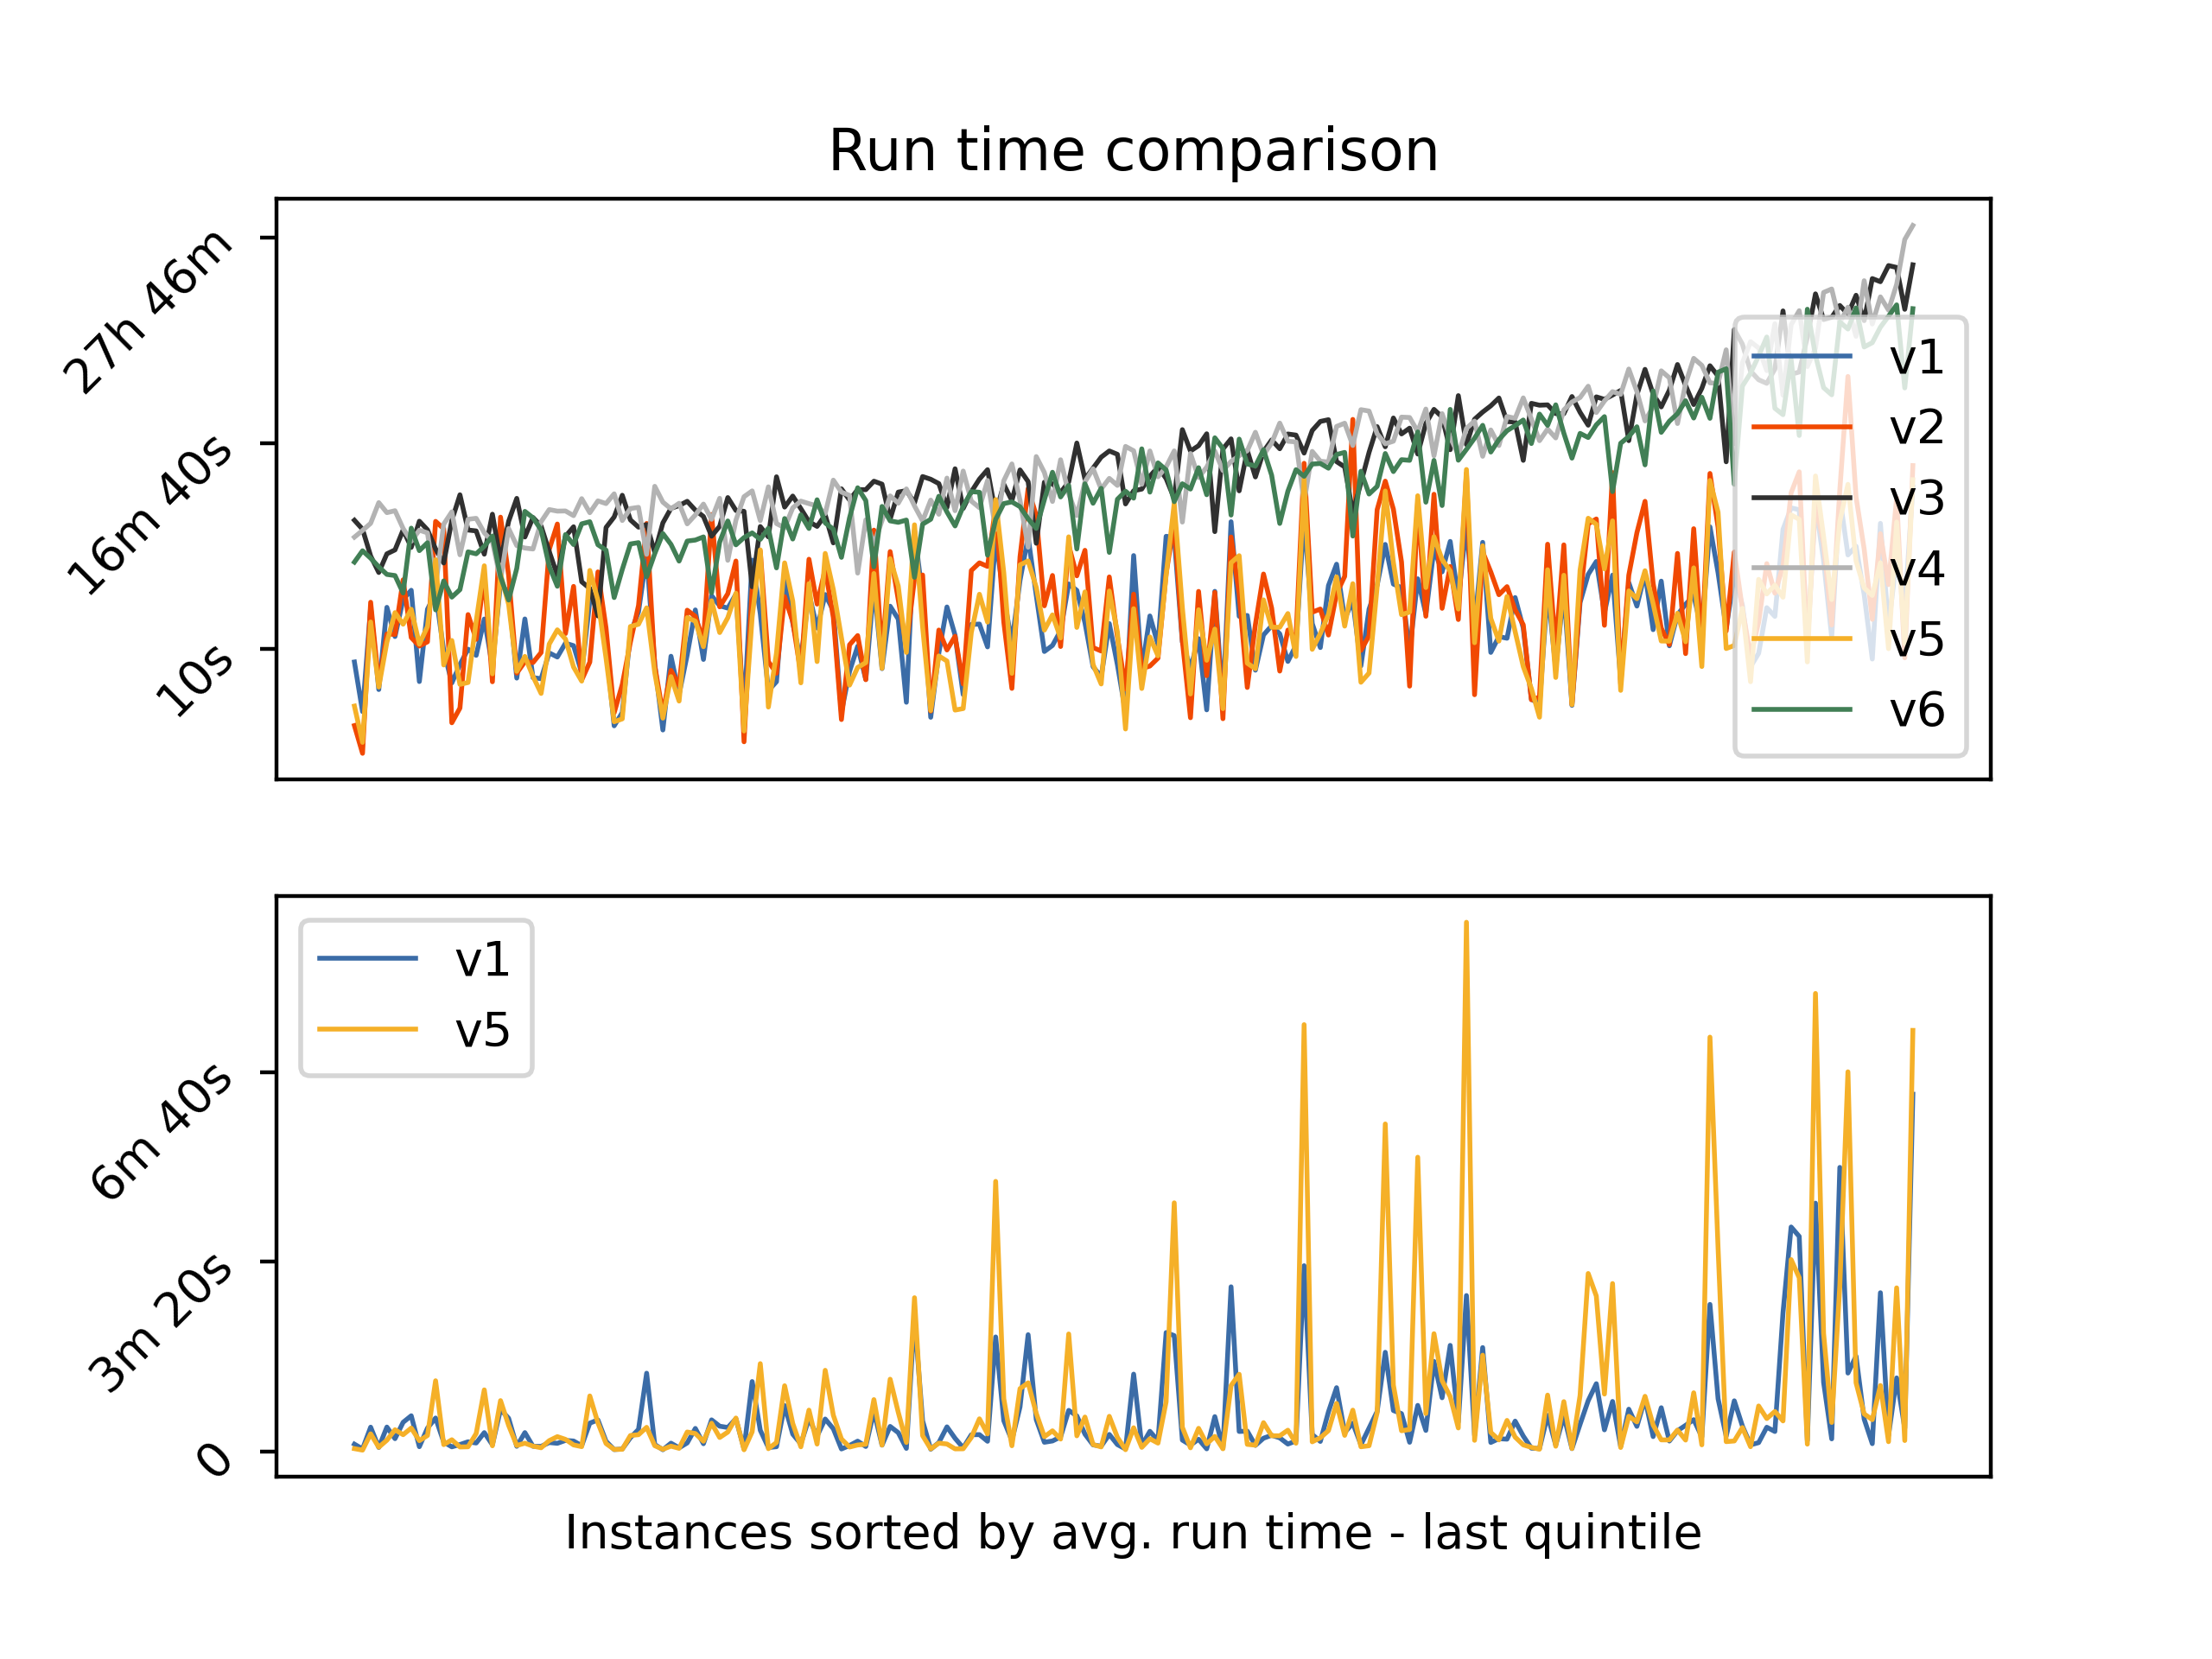
\includegraphics[width=12cm]{../resources/run_time_comparsion.png}
    \caption{Comparativa de el tiempo de ejecución de todas las versiones. Las instancias, en las abcisas, fueron ordenadas en orden creciente segun el tiempo promedio de ejecución de todas las versiones. En la primer gráfica la escala es logarítmica dado que los valores a comparar oscilan entre pocos segundos y casi treinta horas, en la segunda la escala es lineal. Se tomaron las últimas 200 instancias dado que eran las que presentaban diferencia más notoria.}
    \label{fig:runtimecomparison}
  \end{figure}

  \begin{figure}[h!]
    \centering
    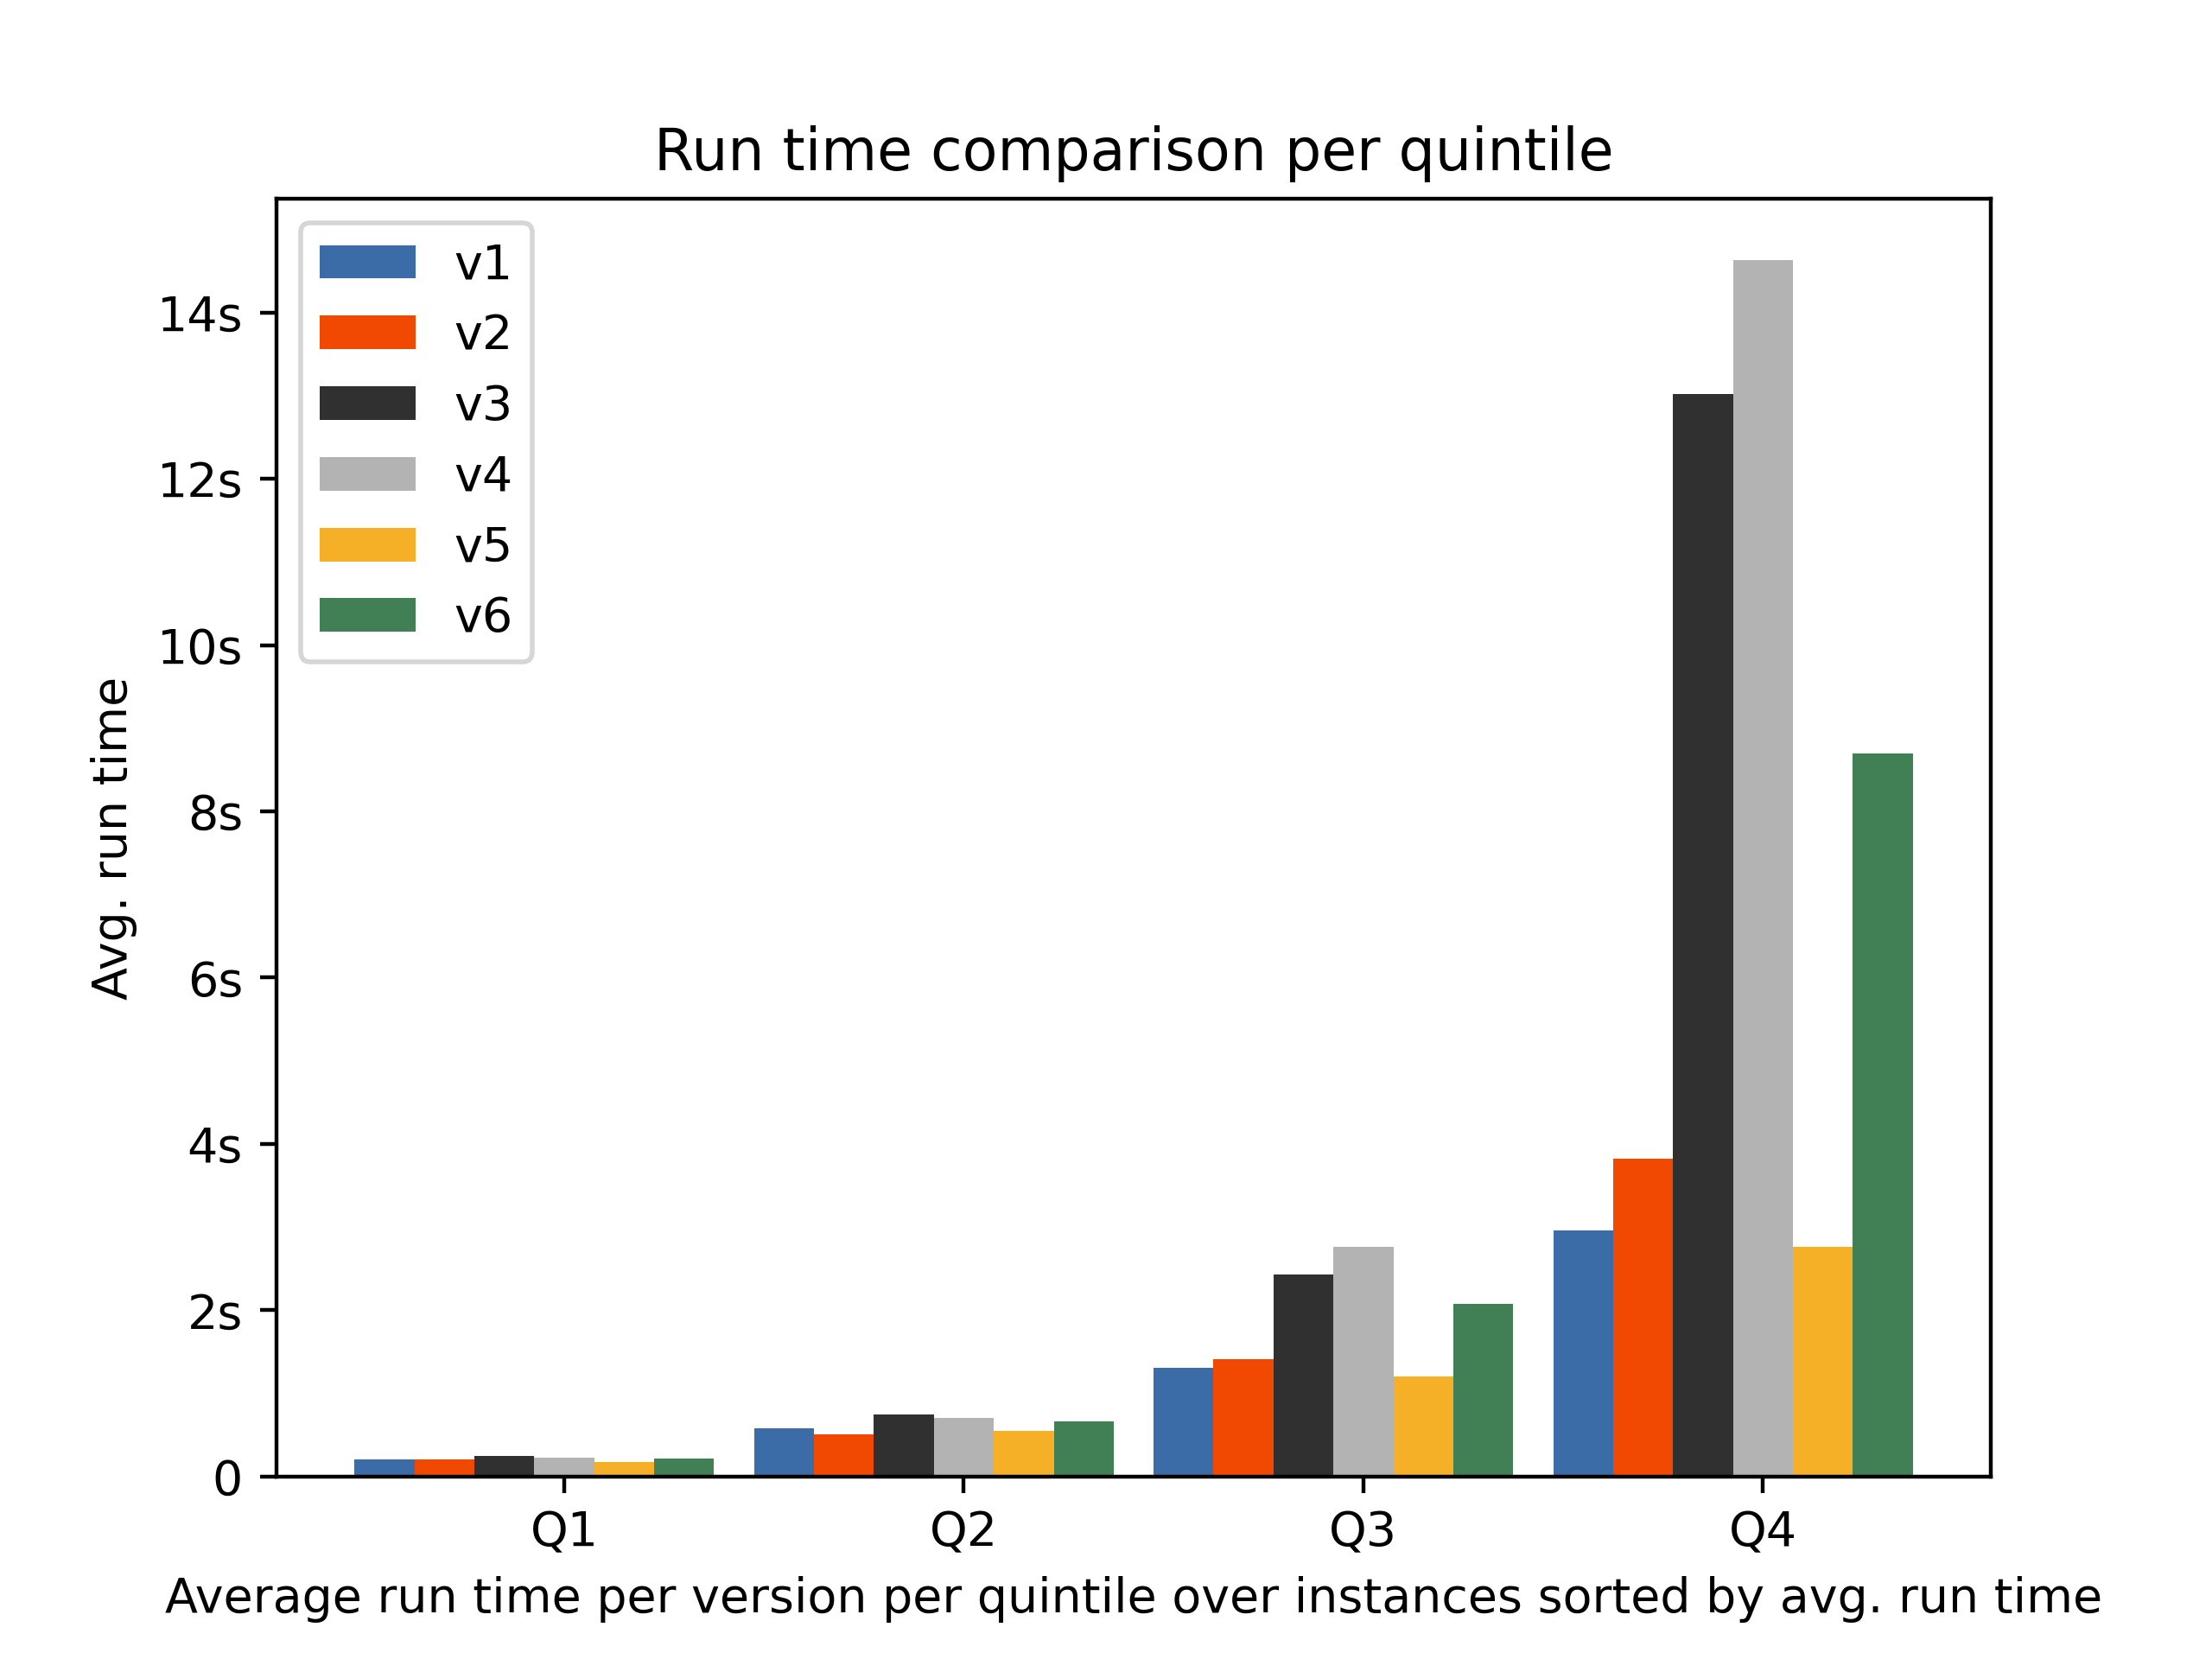
\includegraphics[width=12cm]{../resources/run_time_comparsion_by_quintile.png}
      \caption{Comparativa de el tiempo de ejecución de todas las versiones en tiempo promedio para los cuatro primeros quintiles. El promedio de las ejecuciones es en el tiempo promedio acumulado.}
    \label{fig:firstfourquintiles}
  \end{figure}

  El siguiente aspecto a tener en cuenta es el tiempo de ejecución. El tiempo de ejecución promedio nos da una medida gruesa para comparar y descartar algunas versiones. Las versiones v3, v4 y v6, que utilizan la formulación v1 de $f_k$ tienen un valor significativamente más alto que las otras, que utilizan la otra versión. Es de interés determinar si esta diferencia se da por algun tipo de instancia particular y si alguna versión se desempeña significativamente mejor en terminos de tiempo de ejecución si se quitan las posibles instancias dificiles. En la figura (\ref{fig:runtimecomparison}) se puede comparar el tiempo de ejecución de las versiones en las instancias mas dificiles de las generadas. Las versiones con mayor tiempo de ejecución promedio muestran una clara diferencia con las otras. Tambien se comparan las dos versiones con menor tiempo promedio de ejecución, donde se observa que la v1 es en la gran mayoría de los casos la más rápida. Para las instancias mas sencillas, primeros cuatro quintiles en figura (\ref{fig:firstfourquintiles}) los tiempos de ejecución no varían demasiado entre instancias y solo hacia el quintil cuatro se notan algunas diferencias aunque estas son de algunos segundos.

  Considerando el tiempo de ejecución promedio y el hecho de que no hubo incumplimientos en los chequeos se vislumbra mejor la implementación con la segunda version de formulación de $f_k$ con variables de holgura $r$, es decir la formulación v1. Sin embargo, para solucionar la diferencia en demanda transferida total obtenida en una instancia se decidió solucionar este problema y realizar la comparación nuevamente, esta vez con las versiones v1, v2 y v3.

  Para solucionar la diferencia en demanda transferida se agregó un parámetro que disminuye el efecto de las variables de resto $r$ en la función objetivo de la version v1 y se ejecutaron nuevas pruebas, esta vez sobre mil nuevas instancias aleatorias con cuatro infrastructuras lo que le da mayor complejidad, comparando las tres versiones mas rapidas: v1, v2 y v5. Nótese que si bien la v2 tiene incumplimientos estos no implican que la soluciones sean erroneas a los efectos de la demanda transferida.

  % La version v1 modificada sobre las instancias del la primera ronda no genero soluciones con incumplimientos y su tiempo de ejecución promedio
  % fue 10,31 segundos

  \begin{table}[h!]
    \centering
    \caption*{{\bf Resumen de ejecuciones - Segunda ronda}}
    \begin{tabular}{ccc}
      \toprule
      Version & Cant. Incump. & T. Promedio (s) \\
      \midrule
      v1 & 0   & 79.71   \\
      v2 & 119 & 282.11  \\
      v5 & 0   & 207.50  \\
      \bottomrule
    \end{tabular}
    \caption{Comparativa agregada de ejecuciones sobre instancias aleatorias utilizando la segunda ronda de instancias aleatorias sobre la red de Sioux-Falls.}\label{table:resumenreejecuciones}
  \end{table}

  \begin{figure}[h!]
    \centering
    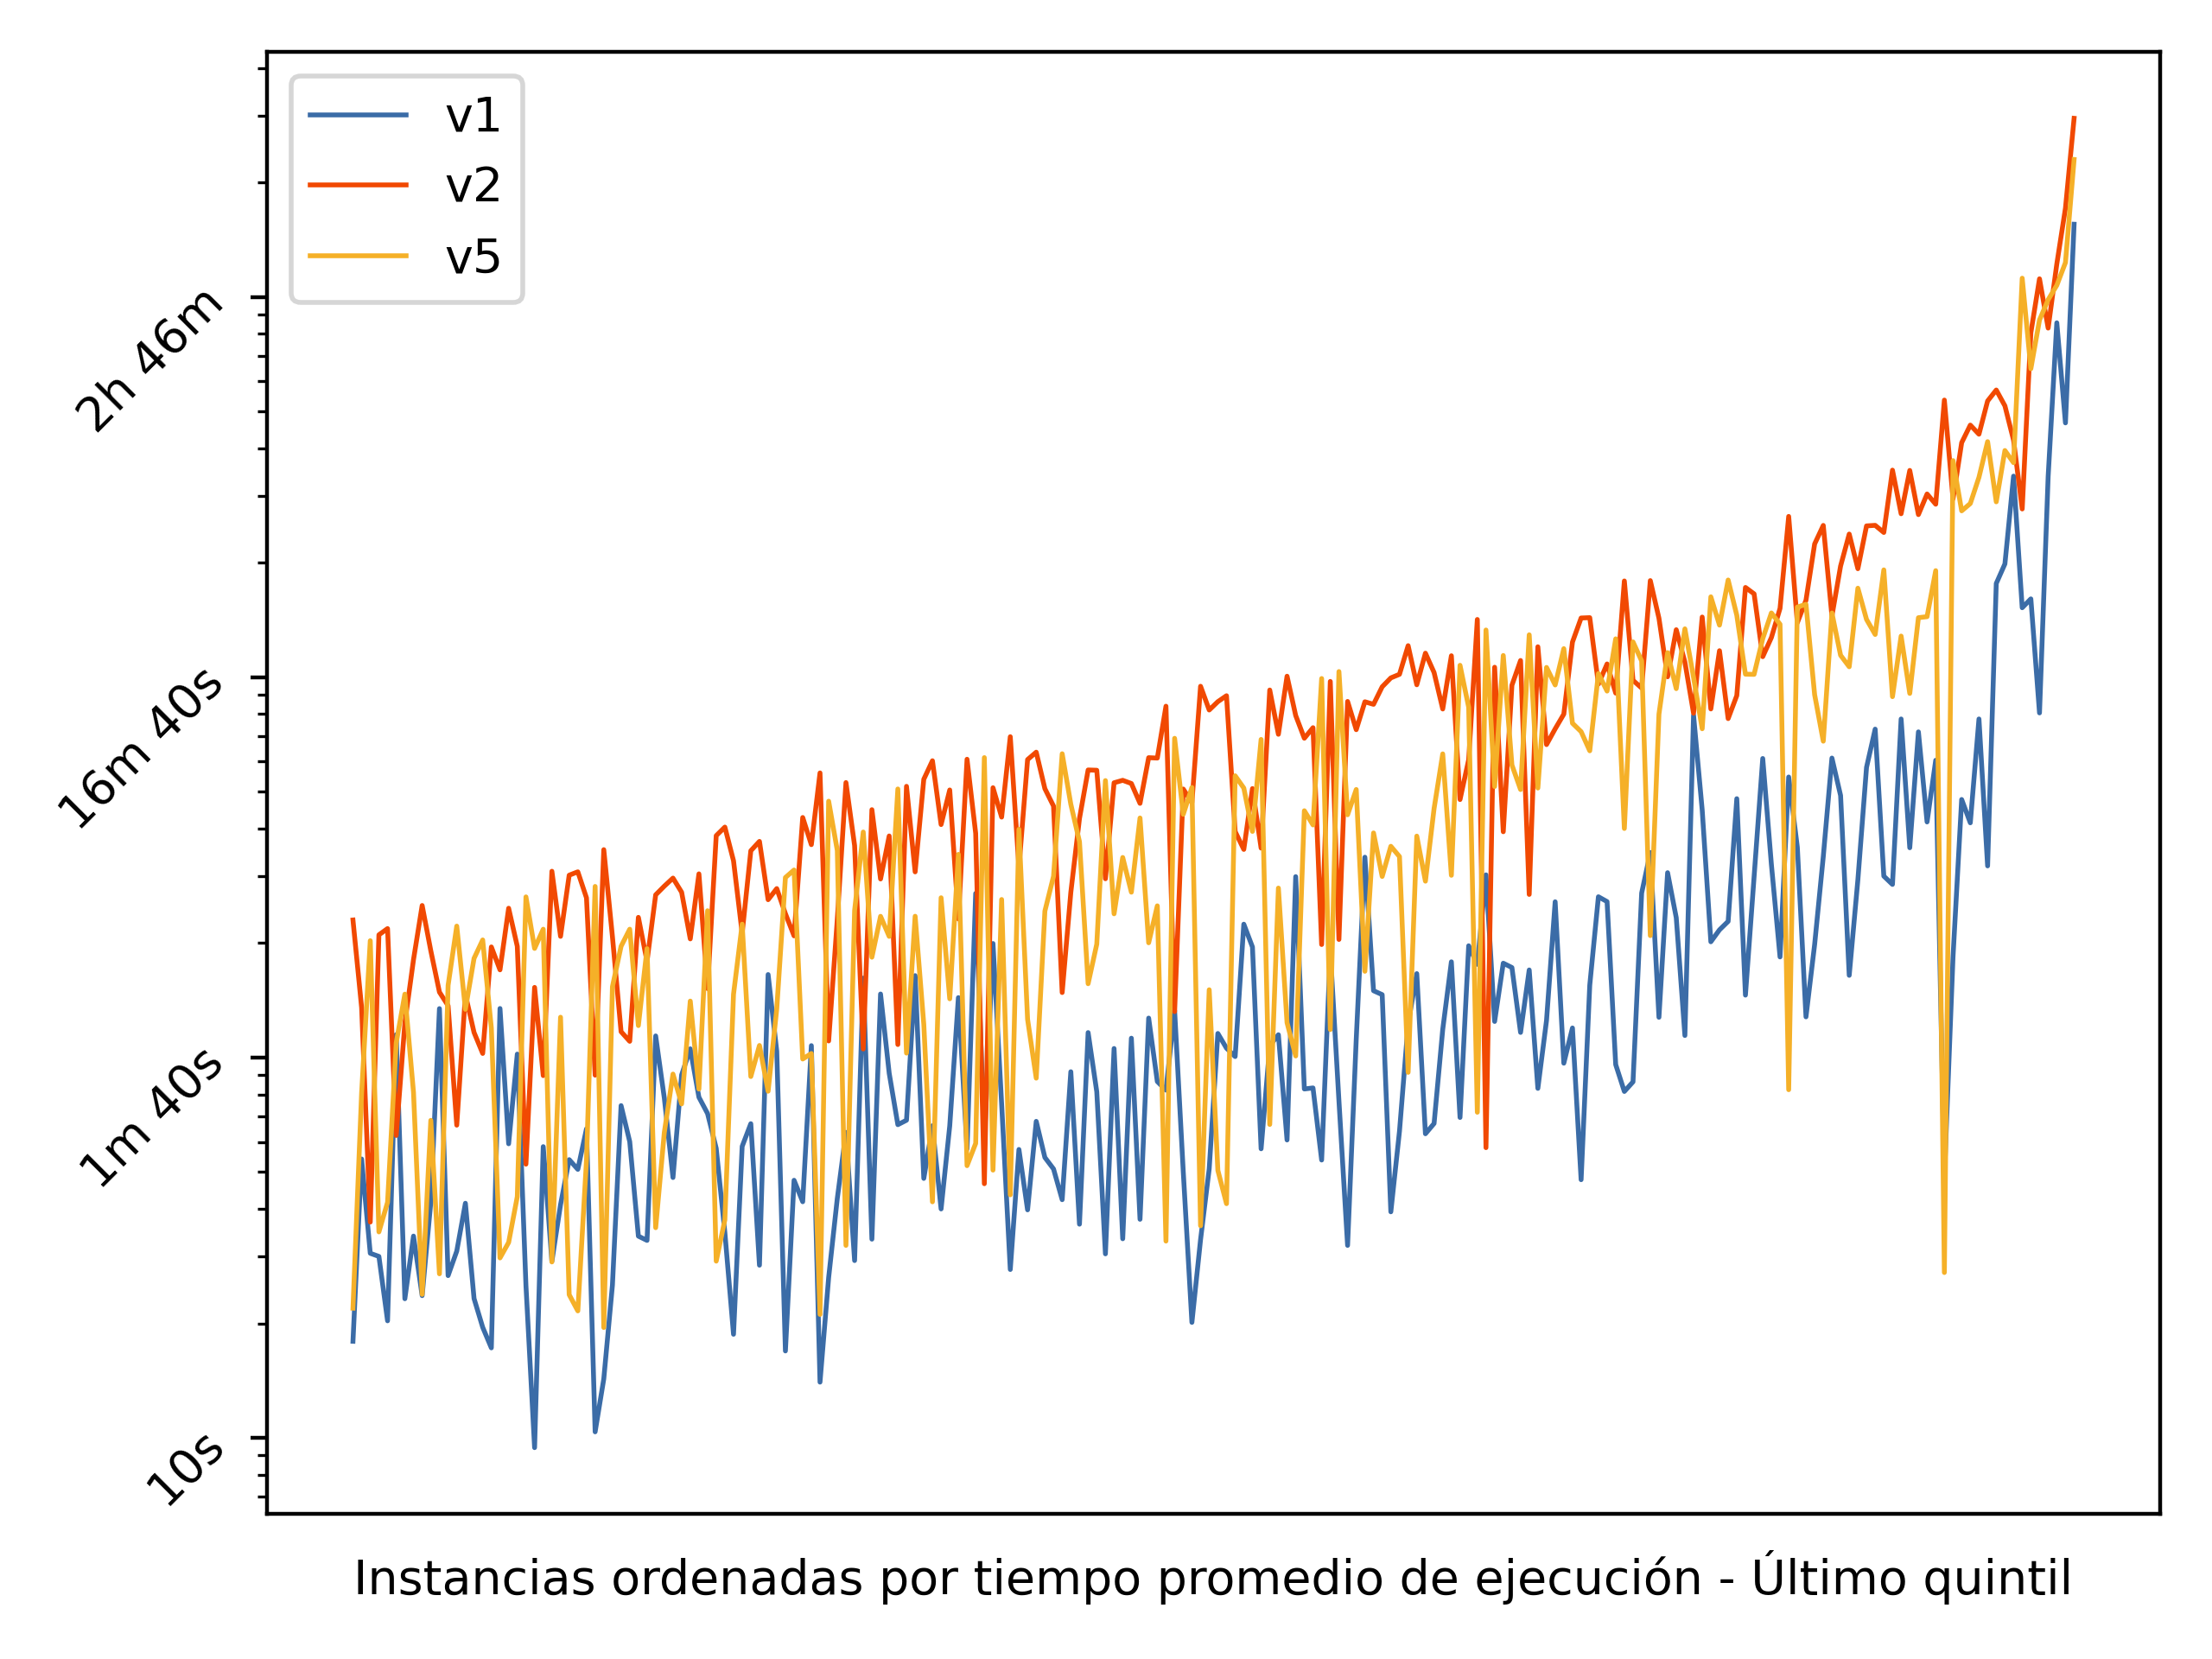
\includegraphics[width=12cm]{../resources/run_time_comparsion_rerun.png}
    \caption{Comparativa de el tiempo de ejecución sobre la segunda ronda de instancias en los tres mejores modelos de la primera. La escala es logarítmica en el eje de las ordenadas.} \label{fig:runtimecomparisonrerun}
  \end{figure}

  \begin{figure}[h!]
    \centering
    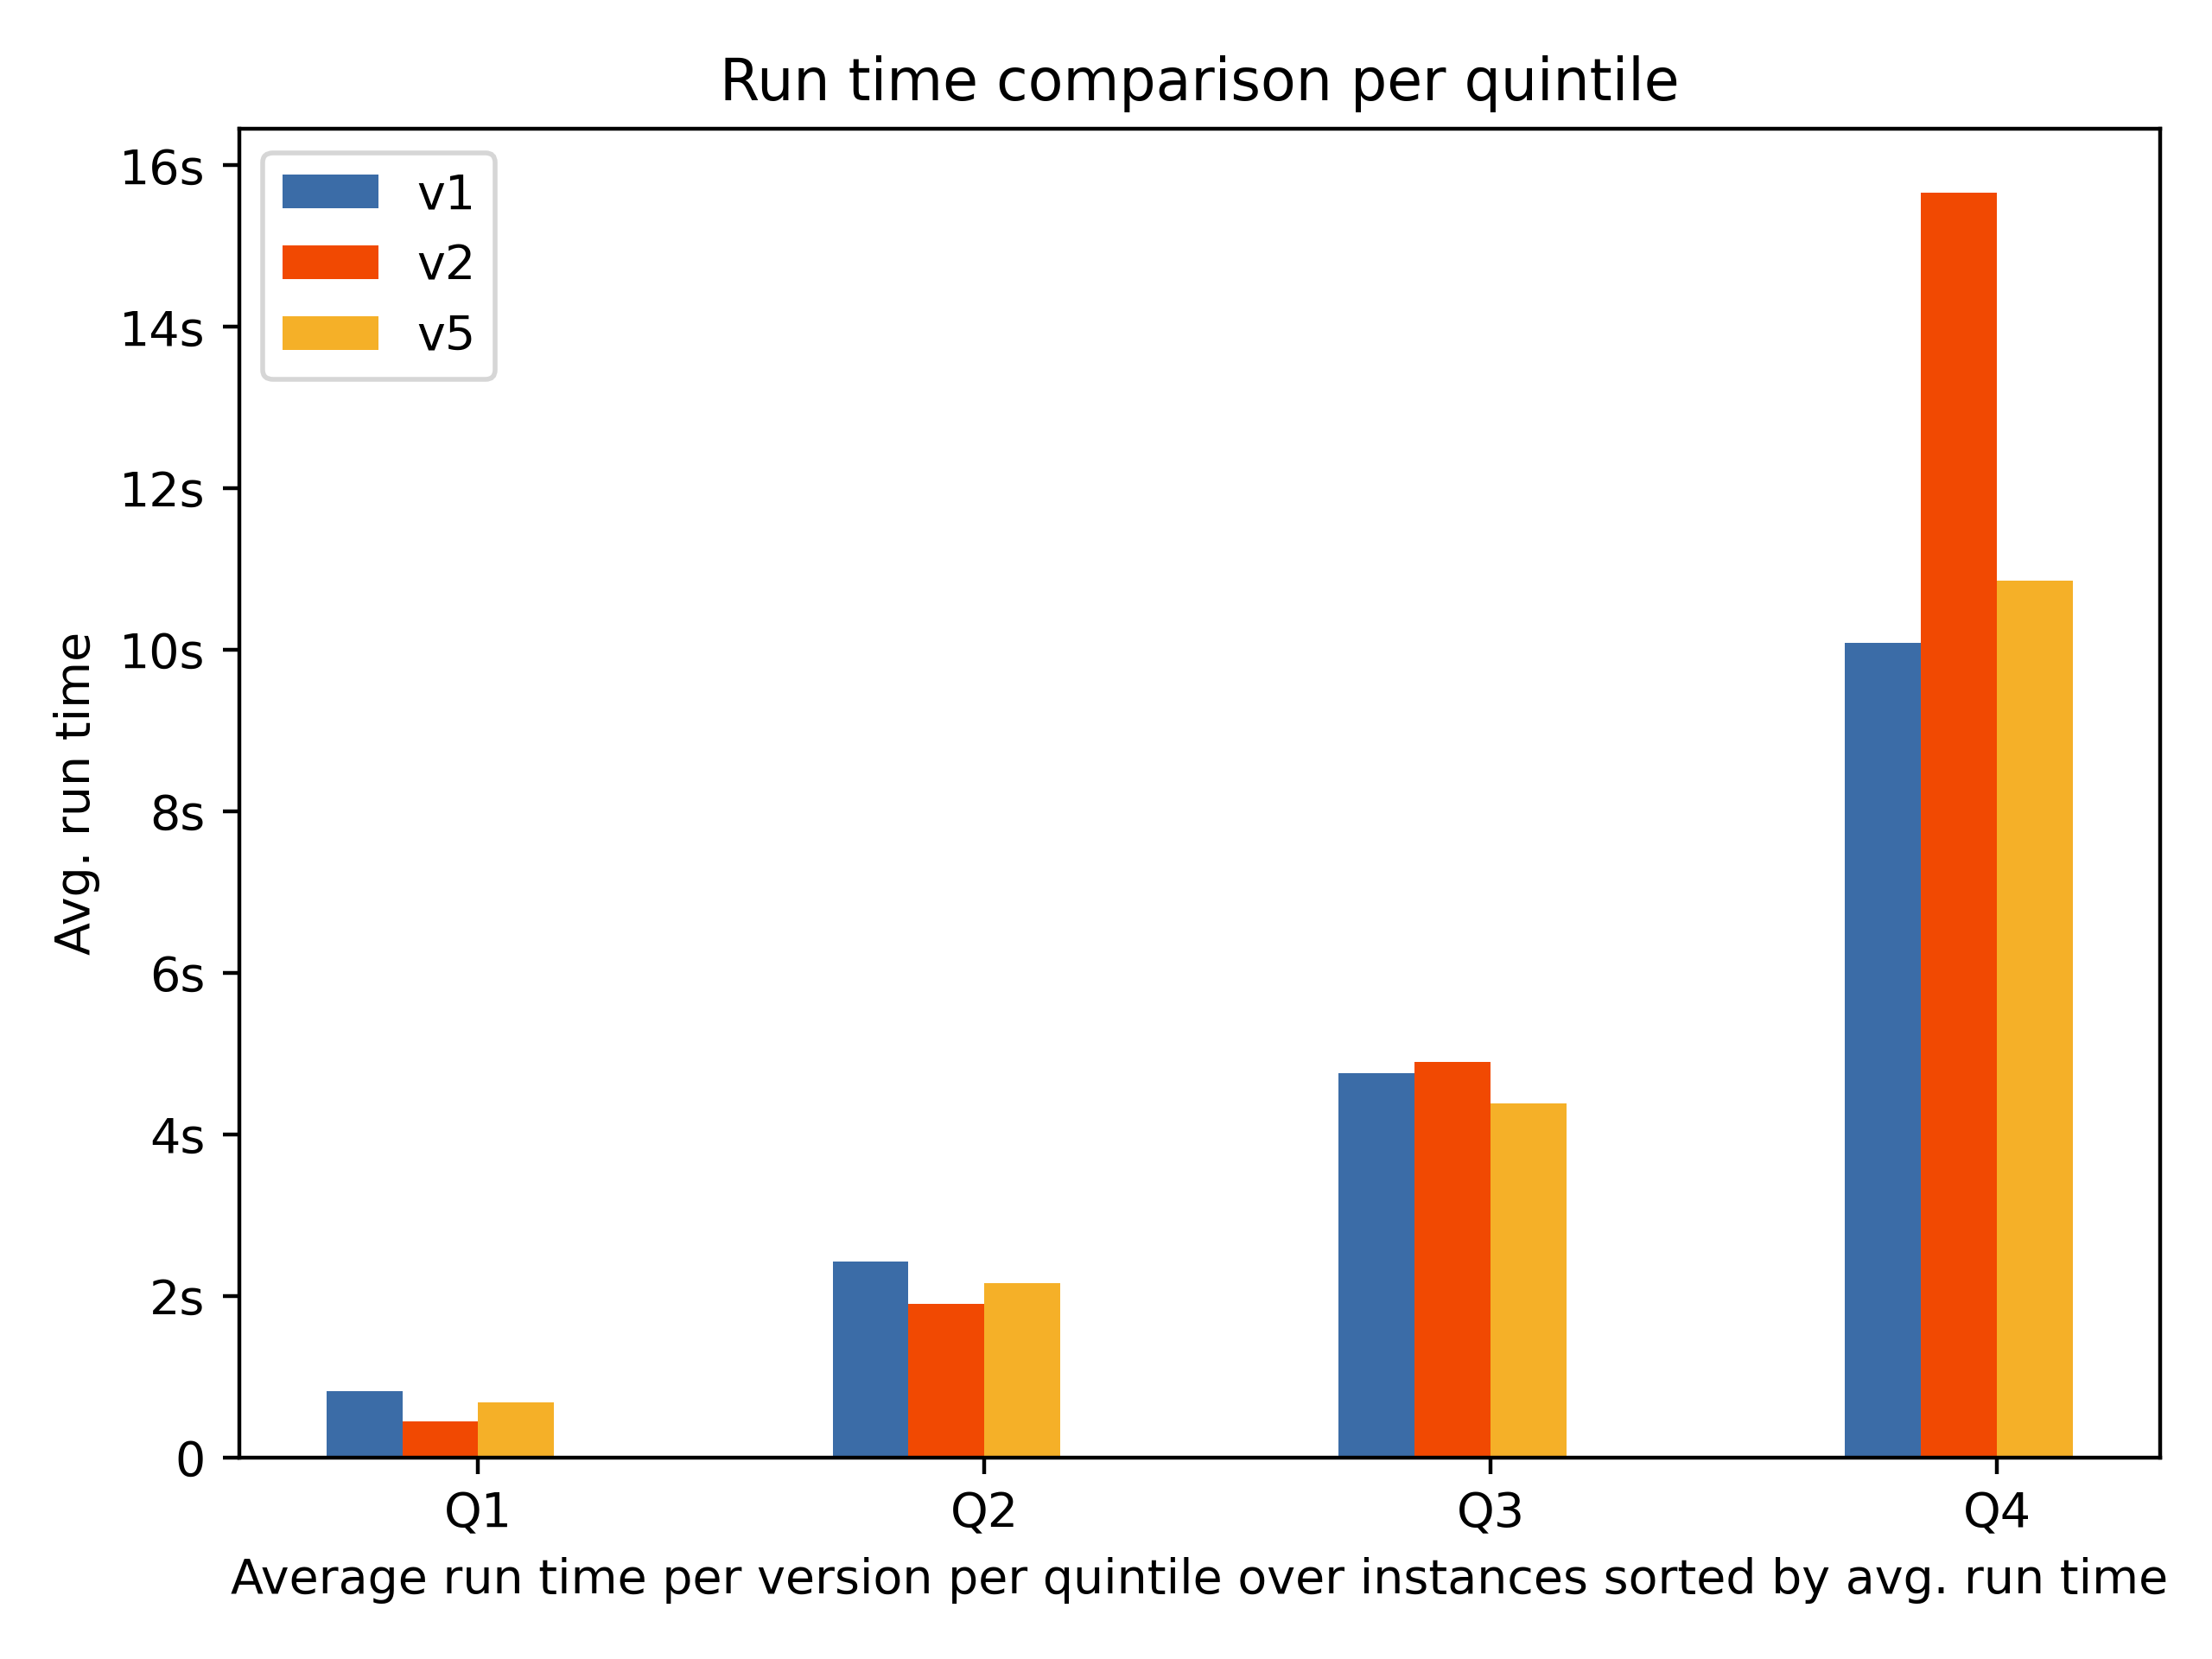
\includegraphics[width=12cm]{../resources/run_time_comparsion_by_quintile_rerun.png}
    \caption{Comparativa de el tiempo de ejecución sobre la segunda ronda de instancias en los cuatro primeros quintiles. Las instancias fueron ordenadas por tiempo promedio de ejecución.} \label{fig:firstfourquintilesrerun}
  \end{figure}

  Los resultados de las nuevas corridas se encuentran en la tabla (\ref{table:resumenreejecuciones}) y las figuras (\ref{fig:runtimecomparisonrerun}) y (\ref{fig:firstfourquintilesrerun}). Se puede observar que se mantiene el comportamiento anterior y el v1 sigue siendo más rápido, también se observa que el desempeño el v5 se degadó de peor manera tomando como referencia las otras dos versiones. En los nuevos resultados no hubieron diferencias en términos de demanda total transferida y se verificó correctamente que el problema fué solucionado en la instancia de la primera ronda. Dados los resultados, se decidió continuar el resto de este trabajo con la version v1 de la formulación.

  \subsection*{Especificación de datos}

  La formulación requiere la presencia de parámetros que en la práctica son de dificil o no son facilmente especificables en términos de un valor escalar. La cantidad y tipos de infrastructuras de ciclovía varían de país a país tanto en su disponibilidad como en sus costos, aún para el caso de Uruguay es dificil estimar, para las infrastructuras disponibles, sus costos de manera general ya que estos varían de la ubicación, congestión del área de la ciudad, precios de insumos como petroleo y mano de obra, reubicación de paradas de ómnibus y señales de tránsito, como se analiza en el analisis {\it Typical Costs of Cycling Interventions} (\ref{typicalcostsofcylcing}). Podemos simplificar los costos reportados en dicho análisis de manera de poder generalizarlos: decimos que la infrastructura de nivel $i+1$ cuesta el doble que la infrastructura de nivel $i$.

  Los costos de usuarios de atravesar un arco varían en la práctica de factores como ancho de la vía, pavimento, volumen y velocidad del tránstio, entre otros factores, a su vez ponderado por el largo del arco. En el documento {\it Bicycle Level Of Service, Applied Model} (\ref{blos2007}) podemos encontrar el concepto de {\it Bicycle Level of Service} (BLOS), muy utilizado en la literatura, que agrupa estas consideracionen bajo un único valor. Para el cálculo del BLOS se tienen en cuenta los siguientes aspectos, que cuantificados en indicadores luego son utilizados en una fórmula para calcular el puntaje de BLOS que por simplificación se estratifican en 6 niveles del A al F.

  \begin{enumerate}
    \item{Ancho promedio de la banquina, presencia de ciclovía, porcentaje de la vía ocupada por estacionamiento}
    \item{Límite de velocidad de vehículos motorizados}
    \item{Volumen promedio de los vehículos motorizados}
    \item{Porcentage de tránsito pesados (camiones)}
    \item{Condición del pavimento}
  \end{enumerate}

  \begin{table}[h!]
    \centering
    \caption*{{\bf Niveles de BLOS}}
    \begin{tabular}{cccc}
      \toprule
        Nivel & Puntaje BLOS & Infrastructura & Proporción del costo base \\
      \midrule
        A     & $\leq 1.5$   & 5              & 0.4   \\
        B     & 1.5-2.5      & 4              & 0.52  \\
        C     & 2.5-3.5      & 3              & 0.64  \\
        D     & 3.5-4.5      & 2              & 0.76  \\
        E     & 4.5-5.5      & 1              & 0.88  \\
        F     & > 5.5        & 0              & 1     \\
      \bottomrule
    \end{tabular}
    \caption{Niveles de servicio definidos en el BLOS, menor puntaje BLOS es mejor. Para cada nivel se define una infrastructura y su correspondiente proporción de mejora sobre la infrastructura base.}\label{table:blosscores}
  \end{table}

  Tomando como base el puntaje de BLOS estratificado, podemos traducir aproximadamente los puntajes a proporción de mejora de un nivel a otro utilizando la función $C_{infra}(i) = {(28 - 3 (i + 1)) \over 25}$, donde $i \in I = \{0,1,2,\ldots\}$ es la infrastructura, contrario a lo que define el estandar de BLOS, mientras mayor es el índice, mejor es la experiencia de usuario. Suponiendo que F corresponde a infrastructura base (o infrastructura 0), la proporción de mejora de las infrastructuras A-F correspondientes a las 1-5 se pueden observar en la tabla  (\ref{table:blosscores}).

  Para establecer una linea base sobre el comportamiento de las funciones de transferencia de demanda, que por simplicidad, asumimos que todas las $f_k$ se comportan igual $\forall k$. Es decir que $f_k(w_k) = f({w_k \over S^{best}_k})D_k$, donde $D_k$ es la demanda máxima que se puede transferir, $S^{best}_k$ es el costo del camino mas corto sobre la inrfastructura base y $f(x) \in [0, 1], x \in [0, 1]$ modela la proporción de demanda transferida en función de la proporción de $S^{best}_k$ lograda.

  Partimos del trabajo {\it Performance evaluation of extreme bicycle scenarios} (\ref{shwe2014}) que, analizando una extensiva encuesta realizada en varios países, aproxima a grosomodo una relación lineal entre la proporción de viajes hechos en bicicleta y el largo de infrastructura de ciclovía per cápita. Siguiendo este razonamiento asumiremos la $f$ base como una función lineal decreciente, es decir que, a menor costo de usuario percibido se obtiene mayor atracción de demanda o mayor proporción de viajes en bicicleta. Podemos encontrar en el libro {\it Modeling Transport} (\ref{ortuz2011}) que el comportamiento de la demanda al momento de decidir entre dos modos se comporta como una función con forma de S, logística o sigmoide, por lo tanto esta función también es estudiada. Por completitud se analizarán otras alternativas a $f$ sin demasiado fundamento bibliográfico, una con concavidad positiva y otra con concavidad negativa en el intervalo $[m, 1]$.

  Establecer valores de presupuesto realistas depende altamente de de las condiciones políticas y económicas de cada localidad. Por simplicidad, especificaremos el presupuesto en función del costo total de construcción de la infrastructura de ciclovía inmediatamente mejor a la base construible. Podemos encontrar en la literatura (\ref{rios2015}) y (\ref{shwe2014}) que factores de cubrimiento del 10\% a 40\% del total de la superficie estan dentro de los parámetros normales.

  Finalmente, usaremos la distancia de los arcos como costo de usuario y costo de la infrastructura base. Esto nos da una medida suficientemente simple y general como para usar en cualquier instancia.

  \subsection*{Análsis de sensibilidad}

  En esta sección se analiza cómo afectan las perturbaciones en los datos a las soluciones. Se utilizará la red de Sioux-Falls nuevamente dado que es de un tamaño manejable para realizar todas las ejecuciones en tiempo razonable. Se han dejado los datos de la red fijos y se estudiarán los parámetros especificos del problema, estos son: puntos de quiebre, funciones de transferencia de demanda y presupuesto. La matriz de demanda se toma de Liu 2019 (\ref{liu2019}), con 22 pares origen-destino. Los datos de esta instancia se encuentran en el apéndice.

  En esta sección se busca determinar que características deben tener ciertos parámetros para que la formulaciones devuelva mejores resultados, mas allá de incrementos en el presupuesto. La cantidad de infraestructuras disponibles en una instancia es determinante respecto a la mejora de los caminos, es de esperar que la formulación decida utilizar mejores infraestructuras en los arcos con mayores flujo tanto como el presupuesto lo habilite y la demanda transferida lo amerite. En principio no hay sentido para limitar este número a un valor distinto al mayor posible a menos que el deteriorio en el tiempo de ejecución en comparación a los beneficios en terminos de demanda transferida sea inmanejable. Respecto a los puntos de quiebre se espera que una mayor granuladidad aporte positivamente al valor objetivo logrado aunque, de nuevo, se analizará el deterioro en el desempeño.

  Sobre el grafo y matriz de demanda antedichos, se agregan los siguientes parámetros base, que coinciden de la sección de especificación de datos:

  \begin{description}
    \item[Infrastructuras]: Se utilizán 5 infrastructuras ademas de la base.
    \item[Puntos de quiebre]: Consideramos la función lineal de transferencia de demanda con 5 puntos de quiebre.
    \item[Presupuesto]: Se establece un factor de presupuesto del 80\%, equivalente a cubrir el 40\% de la superficie con ciclovía de un segundo nivel de mejoramiento.
  \end{description}

  \subsubsection*{Perturbaciones}

  Se analizarán las perturbaciones sobre el conjunto de parámetros base aplicando una perturbación de algunos parámetros por vez en lugar de una ejecución de todos las posibles combinaciones de parámetros que implica una gran cantidad de instancias a estudiar.

  En primer lugar se analiza la sensibilidad respecto al factor de presupuesto. Se utilizan valores de 10\%, 80\%, 160\% y 320\% con el objetivo de observar si se cumple la simple intuición de que siempre a mayor presupuesto se obtienen mejores resultados. A su vez se analiza el efecto que tiene la cantidad de puntos de quiebre en los resultados utilizando 5 y 20 puntos para cada presupuesto.

  Luego, se analiza el resultado de aplicar diferentes funciones de transferencia de demanda y cómo afecta el hecho de utilizar diferentes cantidades de puntos de quiebre. Se utilizarán 5, 20 y 50 puntos de quiebre junto a las cuatro funciones mencionadas en la sección anterior. Se definirán los puntos de manera que sean equidistantes en el codominio de $f$, es decir que si hay N puntos, de un punto al siguiente se obtenga una mejora de, aproximadamente, ${1 \over N - 1}$ en la proporción de demanda transferida.

  Como resultado se tienen 36 instancias cuya representacón pre simplifaciones en Simplex son matrices de tamaño 12597x12310 con 562 variables enteras a 14487x14290 con 1552 variables enteras.

  \begin{figure}[h!]
    \centering
    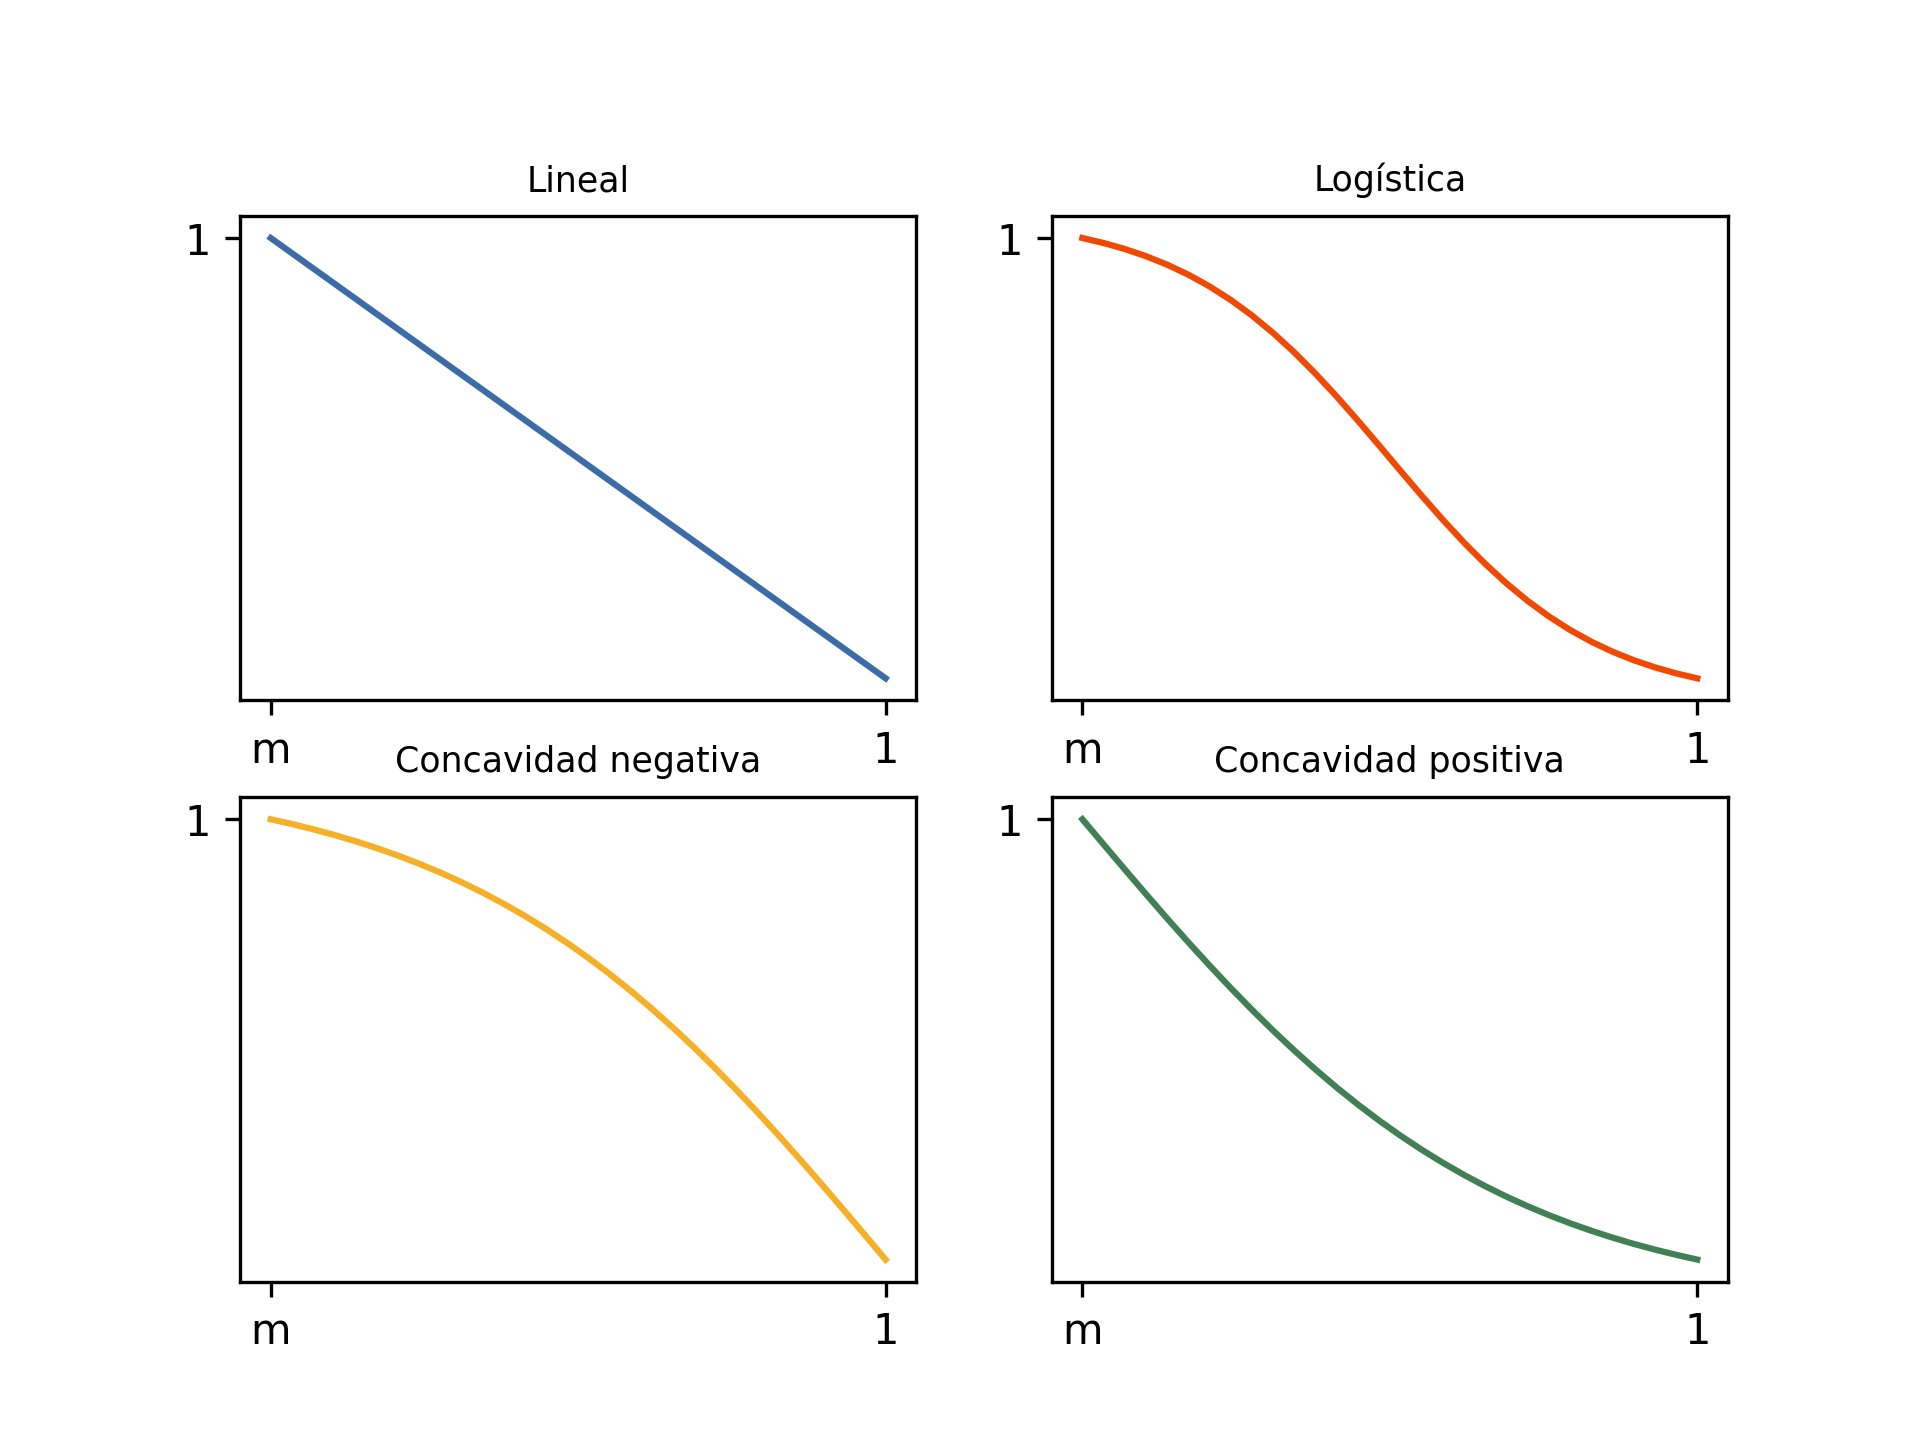
\includegraphics[width=8cm]{../resources/f_catalog.png}
      \caption{Catálogo de funciones $f$ usadas para modelar la transferencia de demanda a la bicicleta. El valor de $m$ varía segun las infrastructuras utilizadas y equivale a la proporción mínima alcanzada por la mejor infrastructura utilizada, es decir $m = min_{i \in I - \{0\}} \{ C_{infra}(i) \}$.}
    \label{fig:fcatalog}
  \end{figure}

  \subsubsection*{Resultados}

  \begin{sidewaystable}
    \centering
    \caption*{{\bf Ejecuciones de sensibilidad de parámetros}}
    \begin{tabular}{cccccc}
        \toprule
        Instancia & Factor de presupuesto & Puntos de quiebre & Funcion $f$ & Demanda transferida (\%) & Tiempo ejecución (\%) \\
        \midrule
        1 & 0,1 & 5 & lineal & 4,65 & 00:00:02 \\
        2 & 0,1 & 20 & lineal & 5,81 & 00:00:11 \\
        3 & 0,1 & 5 & logit & 5,13 & 00:00:01 \\
        4 & 0,1 & 20 & logit & 6,41 & 00:00:08 \\
        5 & 0,4 & 5 & concave down & 32,43 & 00:00:36 \\
        6 & 0,4 & 20 & concave down & 36,49 & 00:07:40 \\
        7 & 0,4 & 50 & concave down & 37,39 & 00:07:29 \\
        8 & 0,4 & 5 & concave up & 15,50 & 00:00:18 \\
        9 & 0,4 & 20 & concave up & 17,05 & 00:09:38 \\
        10 & 0,4 & 50 & concave up & 18,22 & 14:07:09 \\
        11 & 0,4 & 5 & lineal & 18,60 & 00:00:24 \\
        12 & 0,4 & 20 & lineal & 21,32 & 00:06:17 \\
        13 & 0,4 & 50 & lineal & 22,09 & 00:31:55 \\
        14 & 0,4 & 5 & logit & 18,80 & 00:00:27 \\
        15 & 0,4 & 20 & logit & 21,37 & 00:12:35 \\
        16 & 0,4 & 50 & logit & 23,08 & 00:43:53 \\
        17 & 0,8 & 5 & lineal & 32,17 & 00:00:59 \\
        18 & 0,8 & 20 & lineal & 35,66 & 01:26:32 \\
        19 & 0,8 & 5 & logit & 35,47 & 00:00:44 \\
        20 & 0,8 & 20 & logit & 39,74 & 00:05:20 \\
        21 & 1,6 & 5 & lineal & 49,22 & 00:03:22 \\
        22 & 1,6 & 20 & lineal & 53,88 & 00:55:20 \\
        23 & 1,6 & 5 & logit & 58,97 & 00:02:36 \\
        24 & 1,6 & 20 & logit & 63,68 & 00:35:05 \\
        25 & 3,2 & 5 & lineal & 71,71 & 00:00:54 \\
        26 & 3,2 & 20 & lineal & 75,58 & 00:07:49 \\
        27 & 3,2 & 5 & logit & 80,77 & 00:01:33 \\
        28 & 3,2 & 20 & logit & 88,46 & 00:02:39 \\
        29 & 6,4 & 5 & lineal & 94,57 & 00:00:05 \\
        30 & 6,4 & 20 & lineal & 95,74 & 00:00:22 \\
        31 & 6,4 & 5 & logit & 97,44 & 00:00:02 \\
        32 & 6,4 & 20 & logit & 99,57 & 00:00:01 \\
        33 & 12,8 & 5 & lineal & 100,00 & 00:00:00 \\
        34 & 12,8 & 20 & lineal & 100,00 & 00:00:00 \\
        35 & 12,8 & 5 & logit & 100,00 & 00:00:00 \\
        36 & 12,8 & 20 & logit & 100,00 & 00:00:00 \\
        \bottomrule
    \end{tabular}
      \caption{Todas las instancias fueron solucionadas al óptimo en tiempos relativamente cortos a menos de dos instancias cuyo tiempo de ejecución fue más de una hora.} \label{table:sensibilityresults}
  \end{sidewaystable}

  Las instancias fueron ejecutadas con el solver CPLEX con un tiempo máximo de ejecución de 72 horas de wallclock. Los resultados completos se encuentran en la tabla (\ref{table:sensibilityresults}). Se puede observar que a mayor cantidad de puntos de quiebre, fijando la función de transferencia de demanda y el presupuesto, se obtiene mayor transferencia de demanda. A su vez, variar la cantidad de puntos de quiebre parece hacer variar enormemente el tiempo de ejecución en algunos casos sin poderse determinar una relación directa entre la cantidad y la complejidad resultante. Esto tiene sentido ya que la función de transferencia es representada de manera mas precisa. Por otro lado se observa un fuerte impacto en el modelado del comportamiento de la transferencia de demanda respecto a la demanda transferida, si bien las funciones consideradas en este caso pueden ser irreales o exajeradas en sus curvaturas, esto demuestra que es un aspecto clave del problema. Luego, vemos que la demanda transferida en funcion de la cantidad de presupuesto, fijando cantidad de puntos de quiebre y función de transferencia de demanda, escala proporcionalmente hasta cierto punto donde su incidencia empieza a ser cada vez menor, ver figura (\ref{fig:demandtransferbybudgetlinear}).

  \begin{figure}[h!]
    \centering
    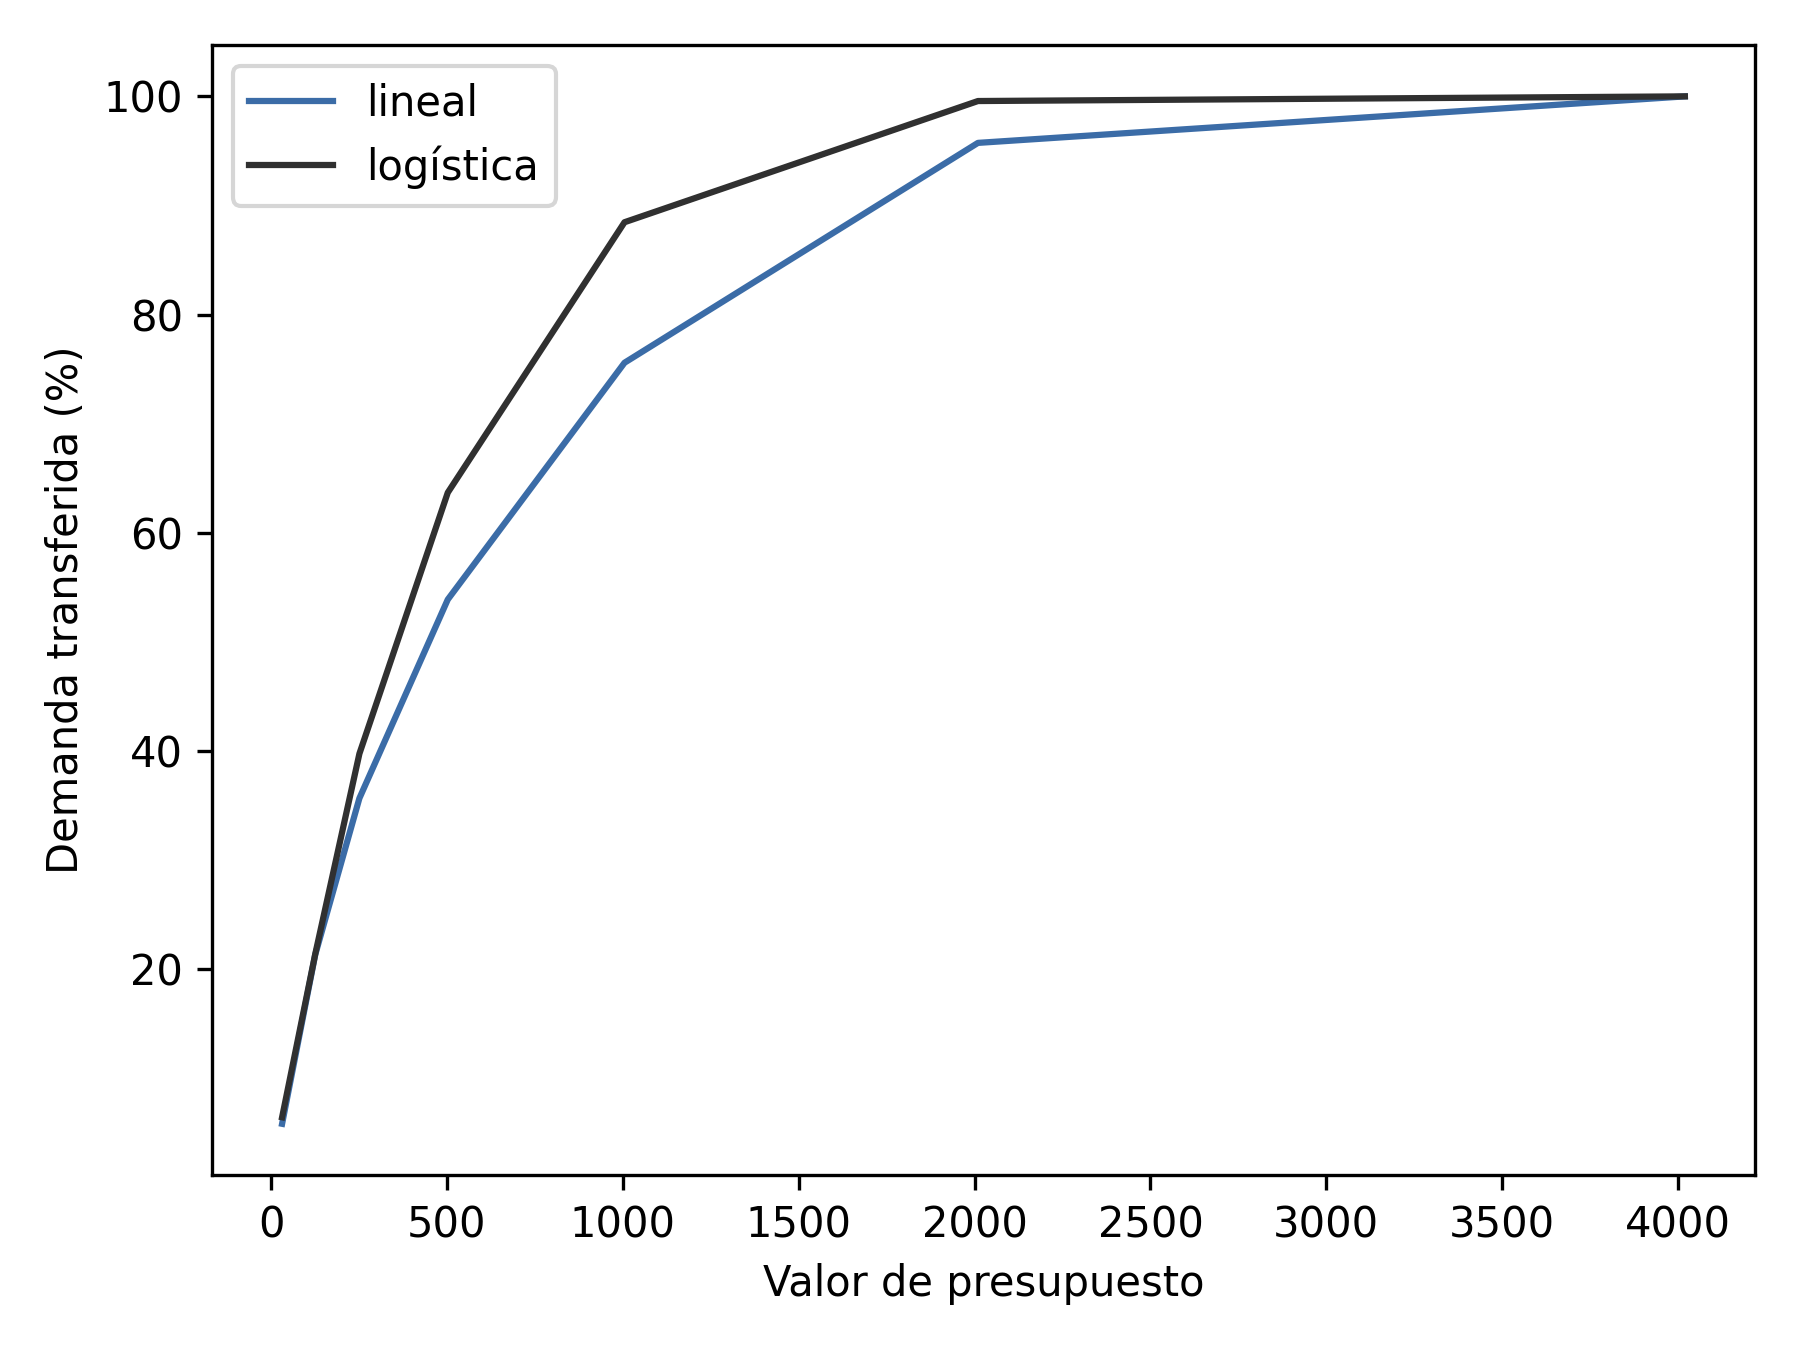
\includegraphics[width=8cm]{../resources/demand_by_budget.png}
      \caption{Porcentage de demanda transferida total en función del presupuesto asignado para Sioux Falls utilizando 20 puntos de quiebre y las funciones de transferencia de demanda lineal y logit. El comportamiento es similar en ambos casos y muestra que la eficiencia de aumentar el presupuesto no es siempre la misma.}
    \label{fig:demandtransferbybudgetlinear}
  \end{figure}

  Respecto a la utilización del presupuesto, se observa que a mayor presupuesto mayor es el porcentaje de gasto en los tipos de infrastructuras mas caras. Se observa que aumentar la cantidad de puntos de quiebre manteniendo presupuesto y función de transferencia fija hace que el gasto en los tipos de infrastructuras varíe, no necesariamente concentrando el gasto en los tipos más caros. El desglose del presupuesto utilizado por infrastructura se detalla en la tabla (\ref{table:sensibilitybudgetusage}) y en la figura (\ref{fig:sensibilitybudgetusage}).

  \begin{sidewaystable}
    \centering
    \caption*{{\bf Presupuesto utilizado por tipo de infrastructura}}
    \begin{tabular}{cccccccc}
        \toprule
        Instancia & Presupuesto & Presupuesto utilizado & Infra 1 (\%) & Infra 2 (\%) & Infra 3 (\%) & Infra 4 (\%) & Infra 5 (\%) \\
        \midrule
        1 & 31,4 & 31 & 35,03 & 63,69 &  &  &  \\
        2 & 31,4 & 31 & 9,55 & 89,17 &  &  &  \\
        3 & 31,4 & 30 &  & 44,59 & 50,96 &  &  \\
        4 & 31,4 & 31 & 9,55 & 50,96 & 38,22 &  &  \\
        5 & 125,6 & 125 & 10,35 & 82,80 & 6,37 &  &  \\
        6 & 125,6 & 125 & 3,98 & 89,17 & 6,37 &  &  \\
        7 & 125,6 & 125 & 5,57 & 81,21 & 12,74 &  &  \\
        8 & 125,6 & 125 & 2,39 & 23,89 & 41,40 & 31,85 &  \\
        9 & 125,6 & 125 & 7,17 & 12,74 & 47,77 & 31,85 &  \\
        10 & 125,6 & 125 & 2,39 & 27,07 & 50,96 & 19,11 &  \\
        11 & 125,6 & 125 & 15,13 & 33,44 & 50,96 &  &  \\
        12 & 125,6 & 125 & 16,72 & 70,06 & 12,74 &  &  \\
        13 & 125,6 & 125 & 5,57 & 81,21 & 12,74 &  &  \\
        14 & 125,6 & 125 & 3,98 & 44,59 & 38,22 & 12,74 &  \\
        15 & 125,6 & 125 & 5,57 & 11,15 & 70,06 & 12,74 &  \\
        16 & 125,6 & 125 & 2,39 & 36,62 & 60,51 &  &  \\
        17 & 251,2 & 251 & 5,18 & 35,83 & 36,62 & 22,29 &  \\
        18 & 251,2 & 251 & 8,36 & 21,50 & 70,06 &  &  \\
        19 & 251,2 & 251 & 1,99 & 21,50 & 44,59 & 31,85 &  \\
        20 & 251,2 & 251 & 1,19 & 11,15 & 81,21 & 6,37 &  \\
        21 & 502,4 & 502 & 0,40 & 15,92 & 19,90 & 63,69 &  \\
        22 & 502,4 & 502 & 2,39 & 7,56 & 45,38 & 44,59 &  \\
        23 & 502,4 & 501 & 2,19 & 13,93 & 35,83 & 47,77 &  \\
        24 & 502,4 & 502 & 2,79 & 5,57 & 54,94 & 36,62 &  \\
        25 & 1004,8 & 1002 & 0,40 & 4,18 & 13,14 & 19,90 & 62,10 \\
        26 & 1004,8 & 1004 &  & 5,97 & 6,37 & 49,36 & 38,22 \\
        27 & 1004,8 & 1004 & 0,60 & 2,99 & 26,27 & 17,52 & 52,55 \\
        28 & 1004,8 & 1004 & 0,80 & 1,19 & 14,33 & 83,60 &  \\
        29 & 2009,6 & 2008 &  & 0,40 & 4,38 & 3,58 & 91,56 \\
        30 & 2009,6 & 2008 &  & 0,40 & 1,59 & 10,35 & 87,58 \\
        31 & 2009,6 & 2008 & 0,10 & 1,49 & 2,39 & 1,99 & 93,95 \\
        32 & 2009,6 & 2004 &  & 0,60 & 1,59 & 14,73 & 82,80 \\
        33 & 4019,2 & 2719 & 0,17 & 0,20 & 0,80 &  & 66,48 \\
        34 & 4019,2 & 3048 &  & 0,20 &  &  & 75,64 \\
        35 & 4019,2 & 2780 & 0,10 & 0,60 &  &  & 68,47 \\
        36 & 4019,2 & 2994 & 0,05 &  & 0,40 &  & 74,04 \\
        \bottomrule
    \end{tabular}
      \caption{Detalle de presupuesto utilizado por instancia por tipo de infrastructura. Las columnas Presupuesto y Presupuesto Utilizado están en unidades de presupuesto.} \label{table:sensibilitybudgetusage}
  \end{sidewaystable}

  \begin{figure}[h!]
    \centering
    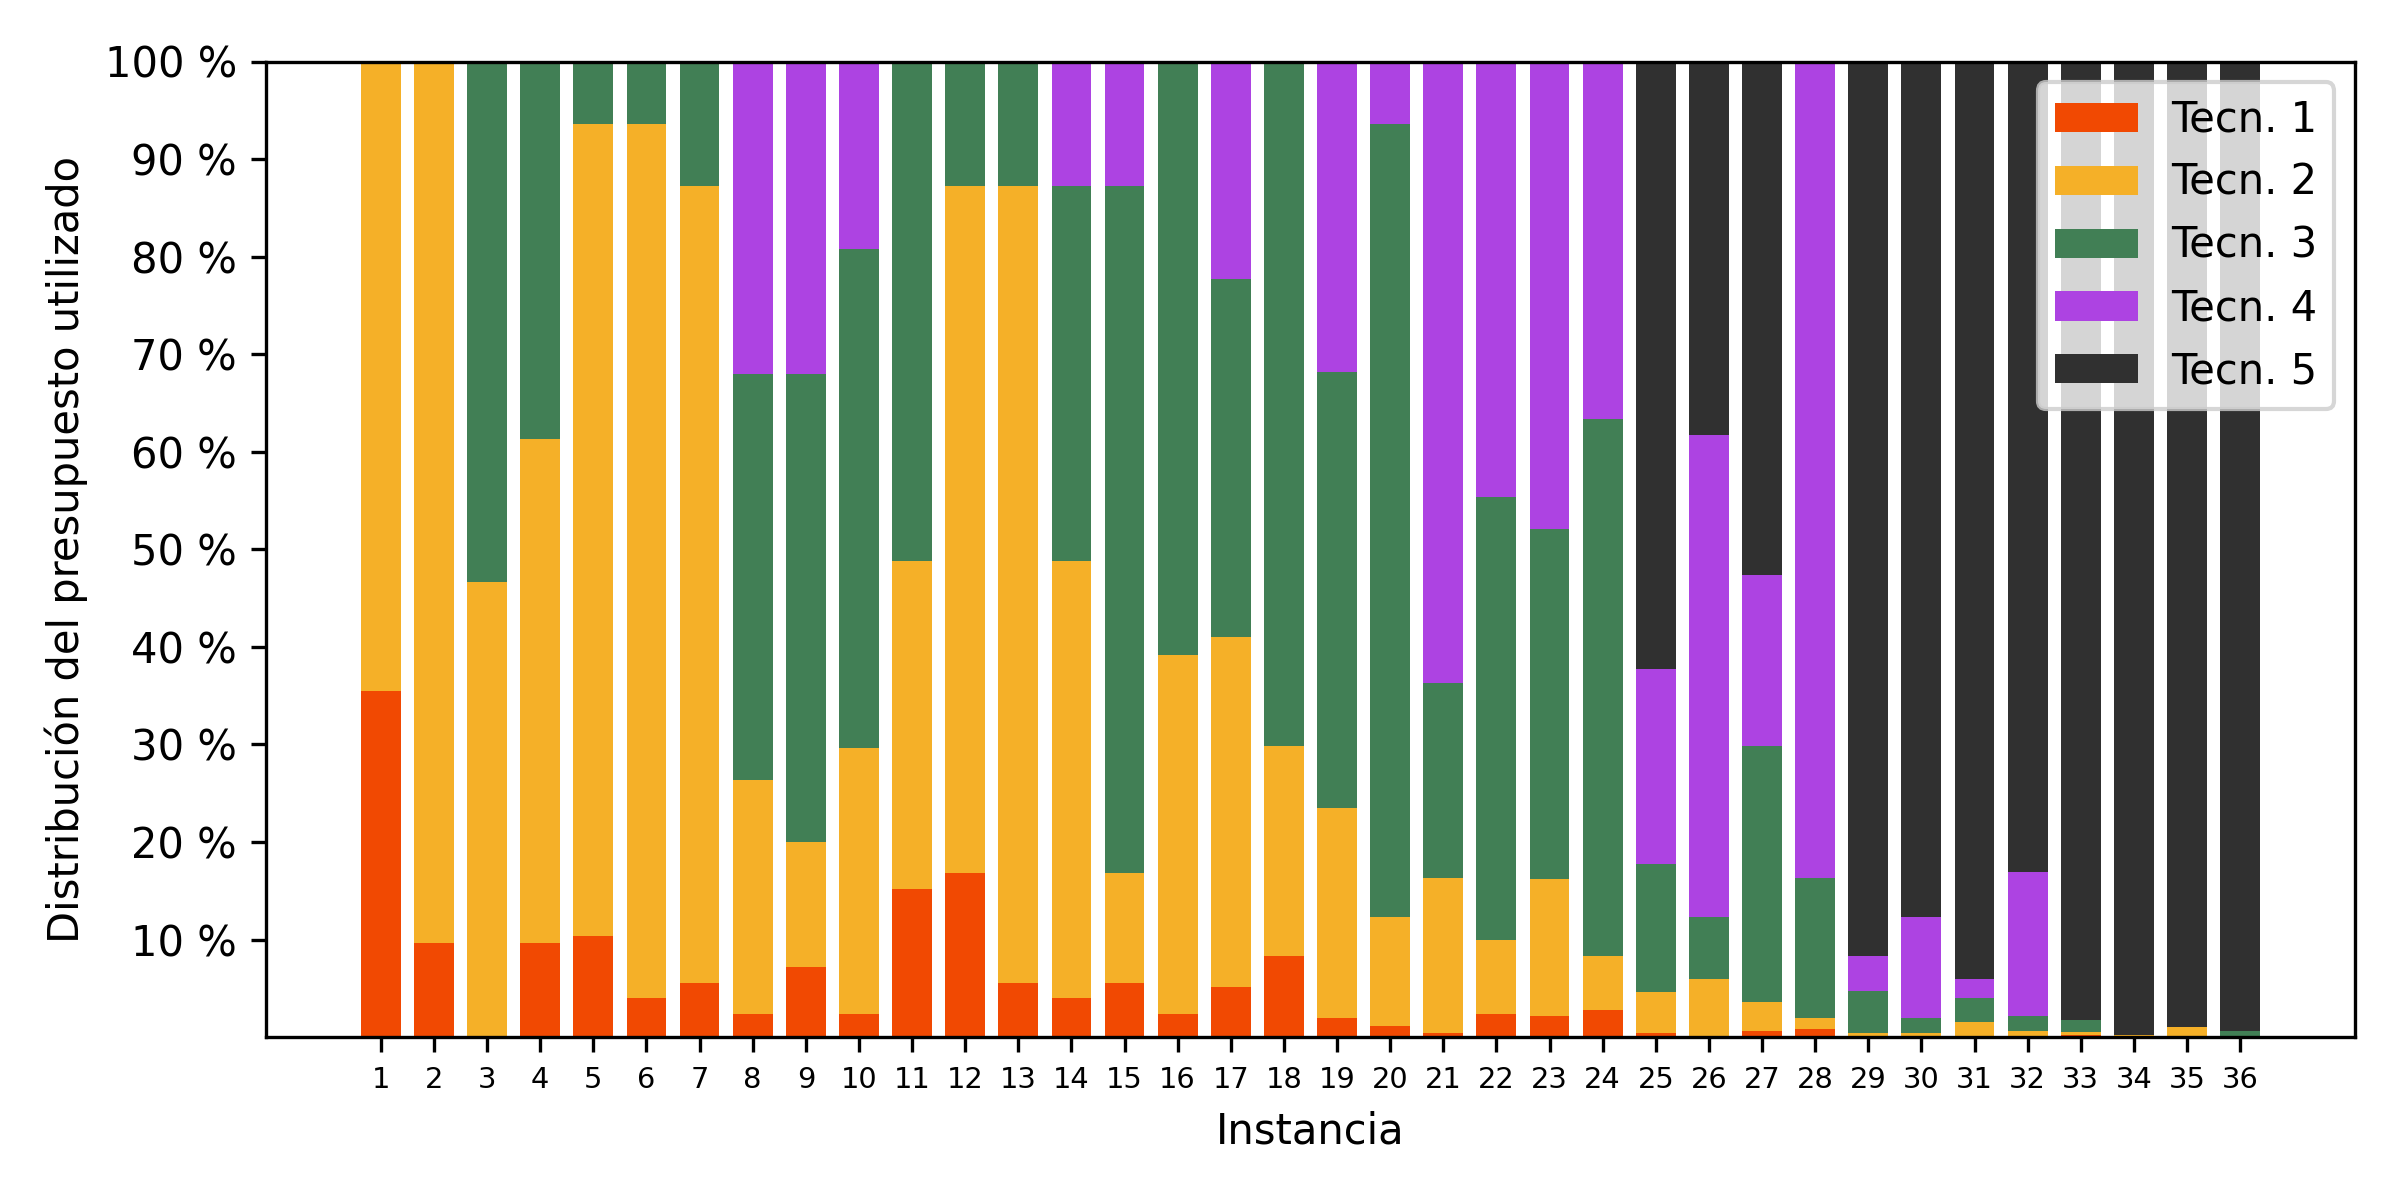
\includegraphics[width=12cm]{../resources/budget_use_by_infra.png}
      \caption{Visualización de la distribución del uso del presupuesto para cada instancia. Los porcentages de uso estan normalizados por el porcentages de presupuesto utilizado.}
    \label{fig:sensibilitybudgetusage}
  \end{figure}

  % TODO: - analisis del presupuesto utilizado por infra
  %       - dibujar grafica de barras stacked con utilizacion de presupuesto porcentual.
  %       - eleccion de puntos de quiebre para varias instancias (dibujar la grafica y algunas lineas verticales)
  %       - dibujar algunos casos interesantes (flujos e infrastructuras)

  \section*{Resultados sobre una instancia realista}

  Se probó la formulación final sobre la ciudad de Montevideo de manera de poder analizar la aplicación práctica del problema sobre datos familiares y realistas. Los datas de la instancia provienen de una red sobre una zonificación de la ciudad y un estudio del comportamiento de la demanda. Esto termina siendo un grafo de 136 nodos y 636 arcos. Respecto a la demanda, consideramos dos conjuntos, uno con 925 pares origen destino, luego de eliminar los elementos con demanda más baja de un total de 6184, y otro con N pares origen destino, considerando de los anteriores, los que quedan a menos de Mkm de distancia, considerado un limite máximo razonable para viajes en bicicleta. Considerando la base dado el tamaño de la instancia y los recursos computacionales disponibles se decidió utilizar 4 infrastructuras, considerando la base, y 10 puntos de quibre. Se probaron las funciones de transferencia de demanda logística y lineal.

  % TODO: Descripción de la instancia
  % - arcos, nodos, centroides
  % - matriz demanda: origen datos
  % - datos de demanda transferida: inventados seguramente

  % TODO: que limite considerar para filtar los 925 pares od?
  %       referencias: red, datos de demanda, por que 925?
  %                    que distancia es un viaje corto?

  \subsubsection*{Comparación frente a otros problemas}

  TODO: aca comparar los resultados con el otro problema de ciclovias trabajado como parte del proyecto de ciclovias.

  \section*{Detalles de implementación}

  Durante el trancurso del proyecto se desarrolló una pequeña biblioteca escrita en Python que facilita la manipulación de datos en torno a las ejecuciones de los solvers. Esto permitió simplificar la tarea de ejecución y manipulación de parametros significativamente, por ejemplo alterar los parámetros de una instancia como la red subyacente o la demanda, generar instancias aleatorias sobre una red o aplicar el problema sobre provistas por OpenStreeMap. También se simplificó el análsis de las soluciones por medio del parseo de los archivos de salida de los solvers. Esto permite el rápido análisis y comparación de un gran volumen de soluciones asi como la representación gráfica de las solcuiones dibujando grafos e infrastructuras.

  La formulación del problema se escribió en el lenguaje MathProg \footnote{http://lpsolve.sourceforge.net/5.5/MathProg.htm} debido a su simpleza y expresividad. Se dió soporte a tres solvers: GLPK \footnote{GNU Linear Programming Kit}, CBC \footnote{\ Coin-or branch and cut MIP solver} y AMPL/CPLEX \footnote{IBM ILOG CPLEX Optimizer}. Los primeros dos son libres y de código abierto y fueron utilizados en la mayor parte del proyecto. GLPK fue tomado como punto de partida y referencia debido a su estabilidad y tiempo en el área. CBC demostró ser mucho más rápido que GLPK (ver figura TODO: comparación de tiempos de de ejecución glpk vs cbc) pero su utilización fué, subjetivamente, ligeramente más complicada debido a que requiere ser compilado especificamente con soporte de MathProg y en su salida no notifica cuando el problema es no factible. Luego se utilizó CPLEX con AMPL para ejecutar la instancias sobre la red de Montevideo.

  \subsection*{Datos de la red}

  Las redes analizadas deben tener una serie de datos asociados de manera que sea posible solucionarlas con el modelo planteado. Para los nodos es necesario (no estrictamente) tener su par de coordenadas, para los arcos, se necesitan los siguientes atributos:

  \begin{description}
    \item[distance]: Distancia o longitud del arco.
    \item[user\_cost]: Costo de usuario de atravesar el arco sobre el grafo base (sin infraestructura o con la infraestructura base $i_0$).
    \item[construction\_cost]: Costo de construcción de la infraestructura base.
  \end{description}

  Luego, si se tienen $N$ infraestructura, para la infraestructura $n$ se calcula el costo de usuario de atravesarla como $user\_cost (-3 (n + 1) + 28) / 25$. El valor del costo de construcción será $2 n construction\_cost$. De ser necesario, pueden especificarse valores particulares de costos de dicha infraestructura para un arco mediante la utilización de los atributos $user\_cost\_n$ y $construction\_cost\_n$.

  \section*{Apéndices}

  \subsection*{Especificación de funciones de transferencia de demanda}

  Las funciones de transferencia de demanda probadas fueron cuatro, ver figura (\ref{fig:fcatalog}). Dada la poca información encontrada en la literatura y la dificultad para obtener estimaciones sobre este comportamiento se decidió probar este conjunto que se cree representativo. Las cuatro funciones se definen parametrizadas por $m$, correspondiente a la proporción de mejora máxima alcanzable por la mejor infraestructura, es decir $m = min_{i \in I - \{0\}} \{ C_{infra}(i) \}$, se definen entonces las funciones en $[m, 1) \rightarrow [0, 1]$ de la siguiente manera:

  \begin{definition}
    Lineal
    \begin{align}
        f(x) = {x -1 \over m - 1}
    \end{align}
  \end{definition}

  \begin{definition}
    Logística
    \begin{align}
        f(x) = {1 \over 1 + e^{2k_m(x - ({1 + m \over 2}))}}
    \end{align}
  \end{definition}

  \begin{definition}
    Concavidad negativa: logística entre $[m, 1)$
    \begin{align}
        f(x) = {2 \over 1 + e^{k_m(x - 1)}} - 1
    \end{align}
  \end{definition}

  \begin{definition}
    Concavidad negativa: logística entre $[m, 1)$
    \begin{align}
        f(x) = {2 \over 1 + e^{k_m(x - m)}}
    \end{align}
  \end{definition}

  El parámetro $k_m$ determina la cuesta de las funciones logisticas y es utilizado para que los valores funcionales en los extremos $m$ y $1$ esten cerca de $1$ y $0$ respectivamente. Fue determinado de manera experimental y se calcula como $k_m = {3 \over 1 - m}$

  \subsection*{Instancia de Sioux Falls}

  Esta instancia se utilizó para las pruebas preliminares y de sensibilidad de parámetros. Aquí se especifican los datos del grafo, costos de usuario sobre la infrastructura base, de construcción en la tabla (\ref{table:siouxfallsgraphdata}) y datos de demanda (\ref{table:siouxfallsdemanddata}). La representación se puede observar en la figura (\ref{fig:siouxfallsapendix}).

  \begin{figure}[h!]
    \centering
    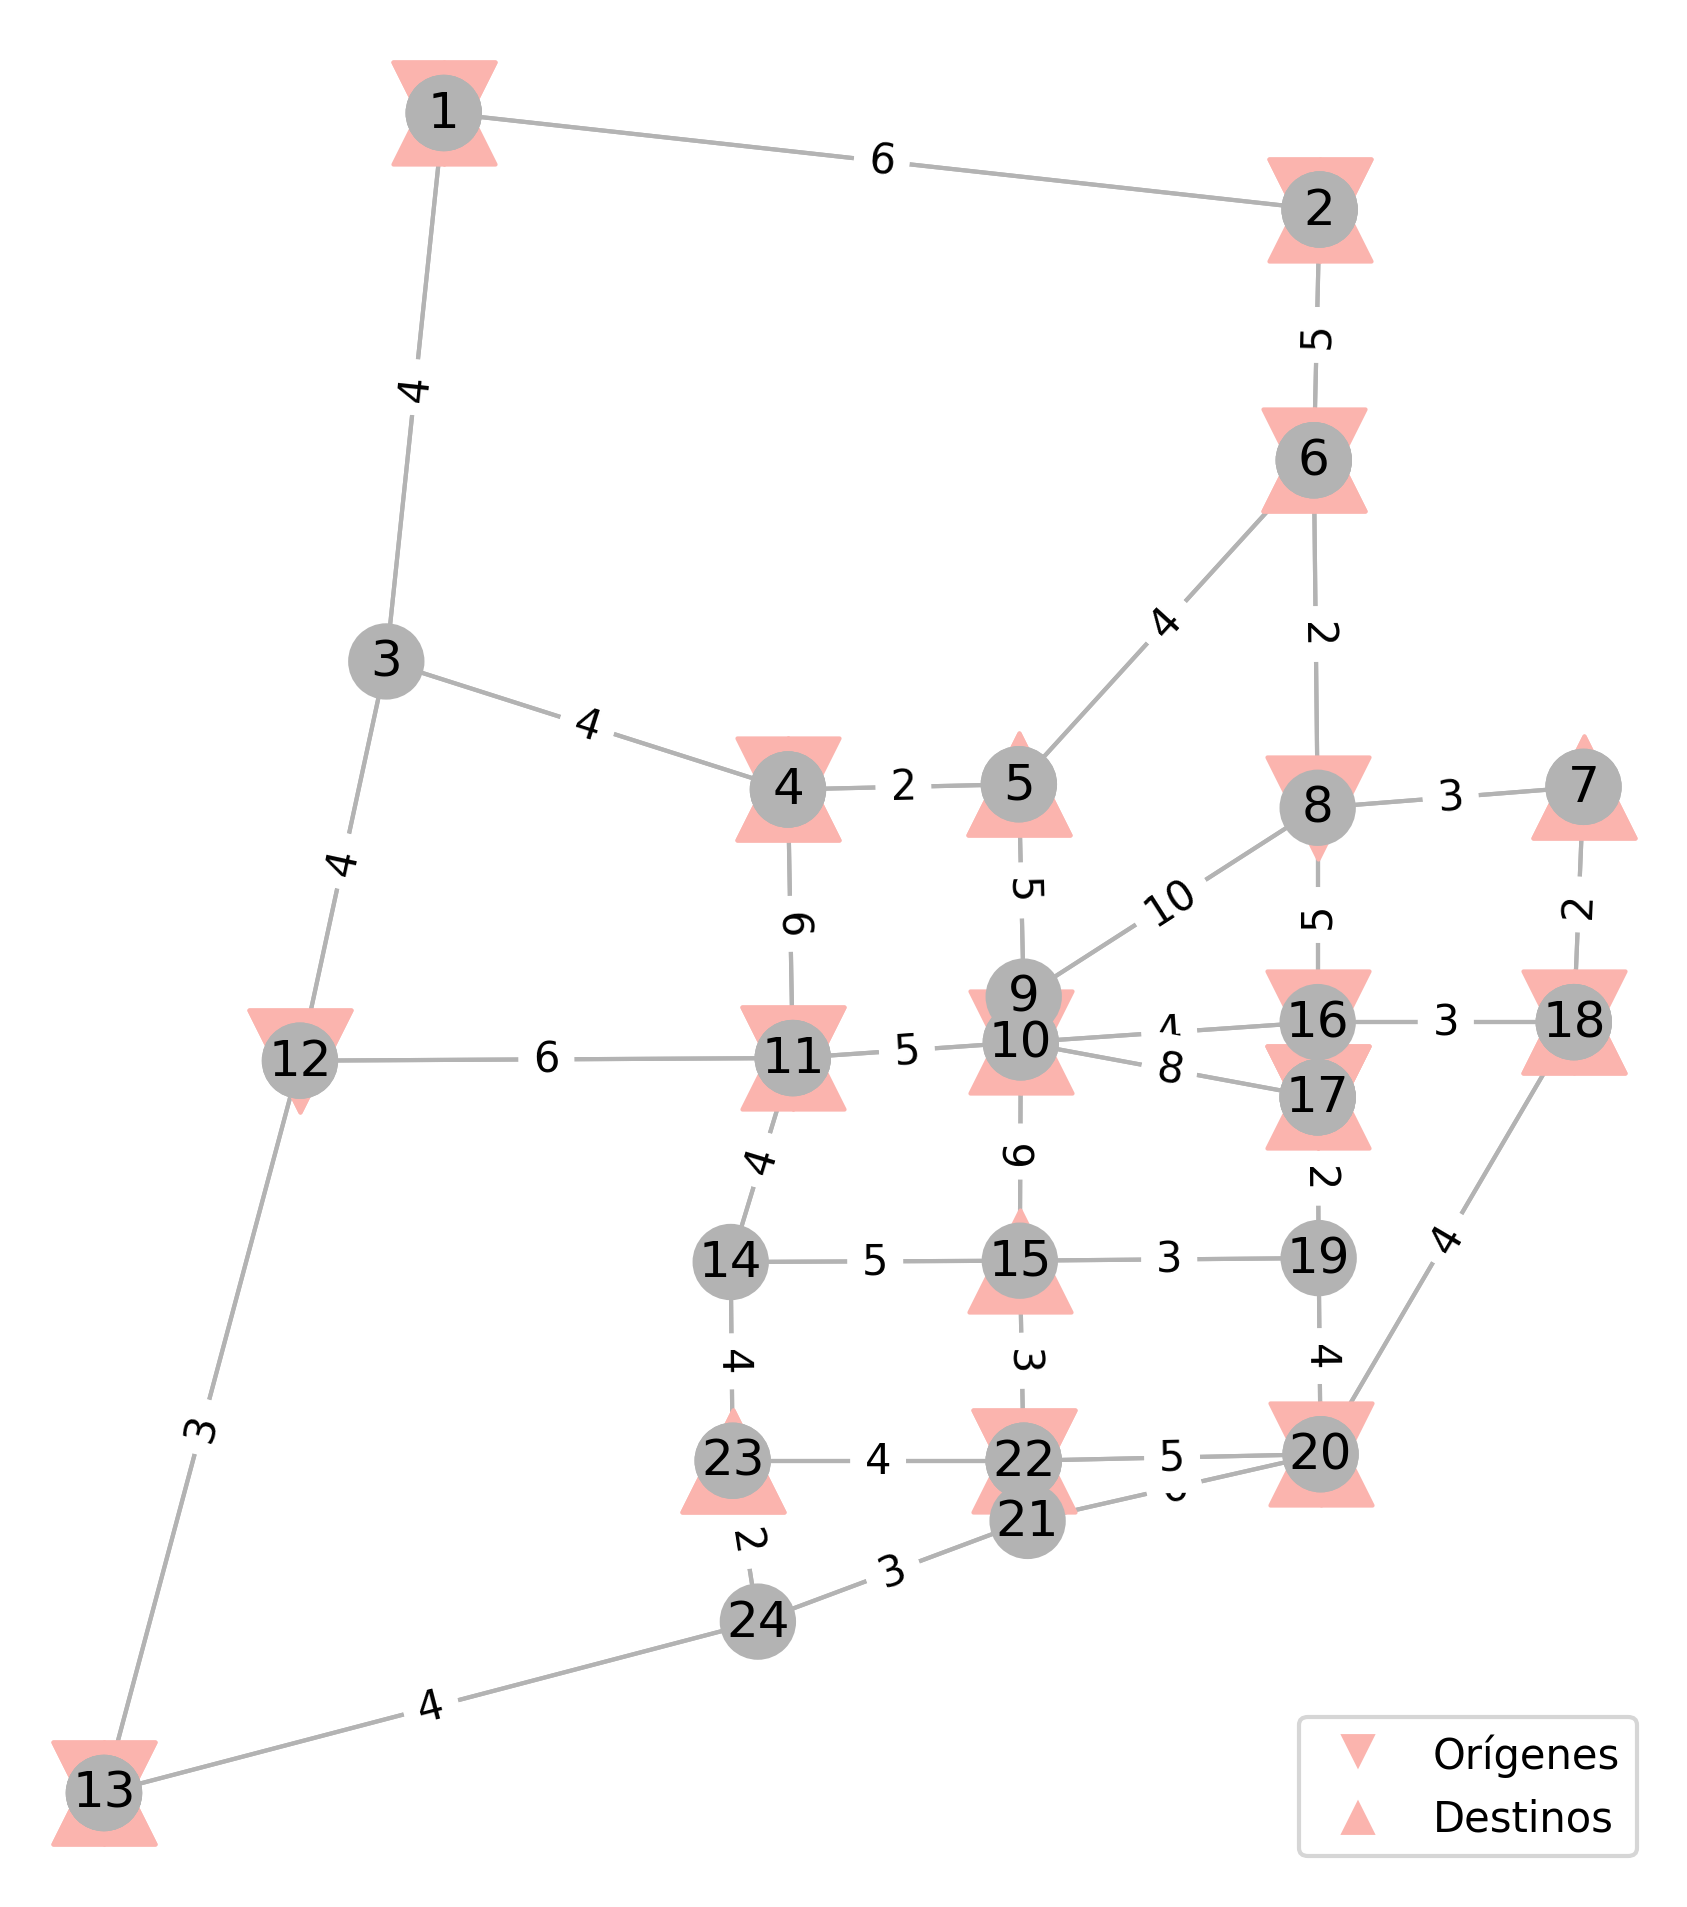
\includegraphics[width=6cm]{../resources/sioux_falls_odpairs.png}
    \caption{Representacón de la red de la instancia de Sioux Falls. Los nodos con triángulo superior azul son origenes y los de triángulo inferior azul destino.}
    \label{fig:siouxfallsapendix}
  \end{figure}

  \begin{table}[h!]
    \centering
    \caption*{{\bf Costo de arcos de la instancia de Sioux Falls}}
    \begin{tabular}{ccc}
      \toprule
        Arco & Costo \\
      \midrule
        (1, 2) & 6 \\
        (1, 3) & 4 \\
        (2, 1) & 6 \\
        (2, 6) & 5 \\
        (3, 1) & 4 \\
        (3, 4) & 4 \\
        (3, 12) & 4 \\
        (4, 3) & 4 \\
        (4, 5) & 2 \\
        (4, 11) & 6 \\
        (5, 4) & 2 \\
        (5, 6) & 4 \\
        (5, 9) & 5 \\
        (6, 2) & 5 \\
        (6, 5) & 4 \\
        (6, 8) & 2 \\
        (7, 8) & 3 \\
        (7, 18) & 2 \\
        (8, 6) & 2 \\
        (8, 7) & 3 \\
        (8, 9) & 10 \\
        (8, 16) & 5 \\
        (9, 5) & 5 \\
        (9, 8) & 10 \\
        (9, 10) & 3 \\
        (10, 9) & 3 \\
      \bottomrule
    \end{tabular}
    \begin{tabular}{ccc}
      \toprule
        Arco & Costo \\
      \midrule
        (10, 11) & 5 \\
        (10, 15) & 6 \\
        (10, 16) & 4 \\
        (10, 17) & 8 \\
        (11, 4) & 6 \\
        (11, 10) & 5 \\
        (11, 12) & 6 \\
        (11, 14) & 4 \\
        (12, 3) & 4 \\
        (12, 11) & 6 \\
        (12, 13) & 3 \\
        (13, 12) & 3 \\
        (13, 24) & 4 \\
        (14, 11) & 4 \\
        (14, 15) & 5 \\
        (14, 23) & 4 \\
        (15, 10) & 6 \\
        (15, 14) & 5 \\
        (15, 19) & 3 \\
        (15, 22) & 3 \\
        (16, 8) & 5 \\
        (16, 10) & 4 \\
        (16, 17) & 2 \\
        (16, 18) & 3 \\
        (17, 10) & 8 \\
        (17, 16) & 2 \\
     \bottomrule
    \end{tabular}
    \begin{tabular}{ccc}
      \toprule
        Arco & Costo \\
      \midrule
        (17, 19) & 2 \\
        (18, 7) & 2 \\
        (18, 16) & 3 \\
        (18, 20) & 4 \\
        (19, 15) & 3 \\
        (19, 17) & 2 \\
        (19, 20) & 4 \\
        (20, 18) & 4 \\
        (20, 19) & 4 \\
        (20, 21) & 6 \\
        (20, 22) & 5 \\
        (21, 20) & 6 \\
        (21, 22) & 2 \\
        (21, 24) & 3 \\
        (22, 15) & 3 \\
        (22, 20) & 5 \\
        (22, 21) & 2 \\
        (22, 23) & 4 \\
        (23, 14) & 4 \\
        (23, 22) & 4 \\
        (23, 24) & 2 \\
        (24, 13) & 4 \\
        (24, 21) & 3 \\
        (24, 23) & 2 \\
         & \\
         & \\
      \bottomrule
    \end{tabular}
    \caption{Costos de usuario y de construcción de la infrastructura 1 por arco de la red, dado que se utilizó el largo del arco, estos costos coinciden.}\label{table:siouxfallsgraphdata}
  \end{table}

  \begin{table}[h!]
    \centering
    \caption*{{\bf Pares origen destino de la instancia de Sioux Falls}}
    \begin{tabular}{ccc}
      \toprule
        Origen & Destino & Demanda \\
      \midrule
        1 & 7 & 34 \\
        1 & 23 & 3 \\
        2 & 13 & 6 \\
        2 & 17 & 4 \\
        4 & 11 & 9 \\
        6 & 1 & 14 \\
        8 & 15 & 10 \\
        10 & 22 & 13 \\
        11 & 5 & 20 \\
        11 & 13 & 1 \\
        12 & 2 & 6 \\
        12 & 10 & 27 \\
        13 & 4 & 5 \\
        13 & 6 & 12 \\
        16 & 18 & 10 \\
        17 & 5 & 9 \\
        17 & 20 & 13 \\
        17 & 23 & 14 \\
        18 & 6 & 16 \\
        20 & 7 & 11 \\
        22 & 4 & 15 \\
        22 & 18 & 6 \\
      \bottomrule
    \end{tabular}
    \caption{Pares origen destino utilizados para la red de Sioux-Falls.}\label{table:siouxfallsdemanddata}
  \end{table}

  \section*{Referencias}

  \begin{enumerate}
      \item{\label{heartrisksuy} MSP (2004). Investigación sobre factores de riesgo cardiovascular en Uruguay.}
    \item{\label{mspphisicalactivityguid} MSP. ¡A MOVERSE! Guia de actividad física.}
    \item{\label{mspsurveyriskfactors} MSP. Encuesta Nacional de Factores de Riesgo de Enfermedades no transmisibles.}
    \item{\label{bardbook} Jonathan F. Bard (1998). Practical Bilevel Optimization, Algorithms and Applications}
    \item{\label{laporte2007} Gilbert Laporte, Ángel Marín, et al. (2007). An Integrated Methodology for the Rapid Transit Network Design Problem}
    \item{\label{lim2021}} Jisoon Lim, Kevin Dalmeijer, et al. (2021). he Bicycle Network Improvement Problem: Optimization Algorithms and A Case Study in Atlanta.
    \item{\label{transportationnetworkrepo} Transportation Networks Repositort \url{https://github.com/bstabler/TransportationNetworks}}
    \item{\label{liu2019} Haoxiang Liu, Haoxiang Liu and Jiancheng Long (2019). Bike network design problem with a path-size logit-based equilibrium constraint: Formulation, global optimization and matheuristic.}
    \item{\label{typicalcostsofcylcing} UK Department for Transport (2017). Typical Costs of Cycling Interventions Interim analysis of Cycle City Ambition schemes.}
    \item{\label{blos2007} Sprinkle Consulting Inc. (2007), Bicycle Level Of Service, Applied Model.}
    \item{\label{shwe2014} Schweizer y Rupi (2014). Performance evaluation of extreme bicycle scenarios.}
    \item{\label{ortuz2011} Juan Ortúzar, Luis Willumsen (2011). Modelling Transport.}
    \item{\label{rios2015} Alberto Ríos, Alejandro Taddia (2015). Ciclo-inclusión en América Latina y el Caribe.}
  \end{enumerate}
\end{document}
